\chapter{Newly Emerged Network Level Sets}
\label{sec:results2}
In this section we study the newly emerged network LSs when individual LSs are not preserved in the network.

In chapter \ref{sec:results1} we focus on conditions for individual LSs preservation in the self-connected cell and the two-cell network. When those conditions are not guaranteed, new network LSs emerge. The goal of this section is to characterize them for different types of networks: homogeneous networks (identical cells), type-\textrm{I} heterogeneous networks (cells belong to the same amplitude and frequency  LS) and type-\textrm{II} heterogeneous networks (cells belong to different frequency and/or amplitude LSs).

We begin characterizing the new network LSs on the connectivity parameter space focusing on connectivity parameter dependencies for the preservation of network attributes. We also investigate the intrinsic parameter space of a single cell and combined parameter spaces involving both connectivity and intrinsic parameters.

\section{The self-connected cell}
As it was shown in chapter \ref{sec:results1}, self-connected cells do not preserve individual LSs. Therefore all network LSs found will be characteristic of the self-connected cell.

Firstly, we study separately the $\lambda-b$ and $\omega-a$ parameter spaces for different values of self-connectivity parameter $\alpha$. Afterwards, we characterize total-generated LSs on the whole intrinsic parameter space and describe parameter dependencies needed to maintain network attributes constant on parameter space.

\subsection{The $\lambda-\alpha$ parameter space}
Individual amplitude LSs are defined in the $\lambda-b$ parameter space and they are total-degenerated since the frequency is also constant along them. To begin with, we consider the $\lambda-b$ parameter space to compare LSs on this parameter space between the self-connected cell and the individual cell.

\begin{Statement}
Amplitude level sets on the $\lambda-b$ parameter space in the self-connected cell are not total-degenerated. The network frequency is not preserved along amplitude level sets on the $\lambda-b$ parameter space.
\end{Statement}

Fig. (\ref{photo12}) shows a representative amplitude LS ($A_{\text{Net}} = 1$) on the $\lambda-\alpha-b$ parameter space. It is also shown the network frequency for each point on the amplitude LS. In particular, when the connectivity parameter $\alpha$ is fixed, it is shown the change in frequency along the amplitude LSs ($A_{\text{Net}} = 1$) on the $\lambda-b$ parameter space.

\begin{figure}[h]
\centering
  \begin{minipage}{0.45\linewidth}
  \centering
    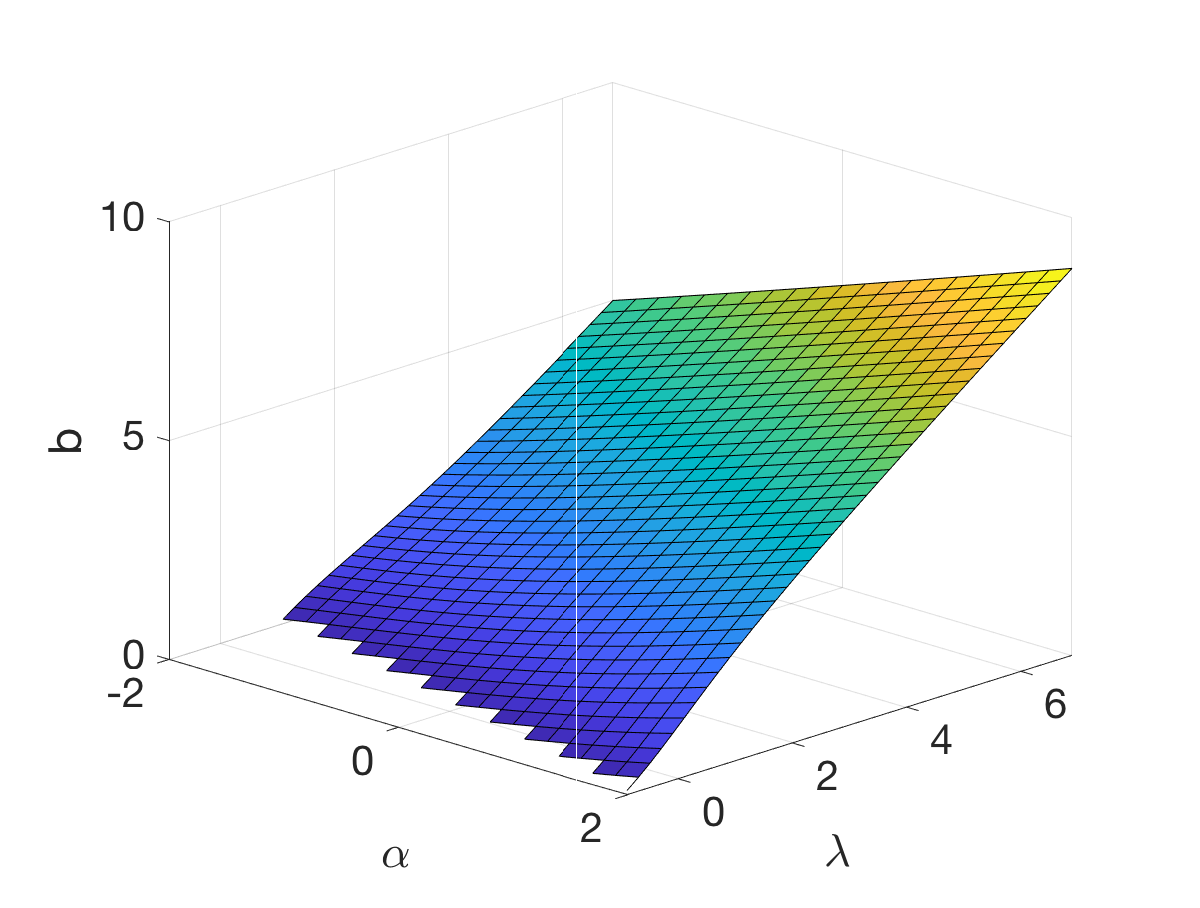
\includegraphics[width=1\linewidth]{Images/photo12_1.eps} 
  \end{minipage} 
  \begin{minipage}{0.45\linewidth}
  \centering
    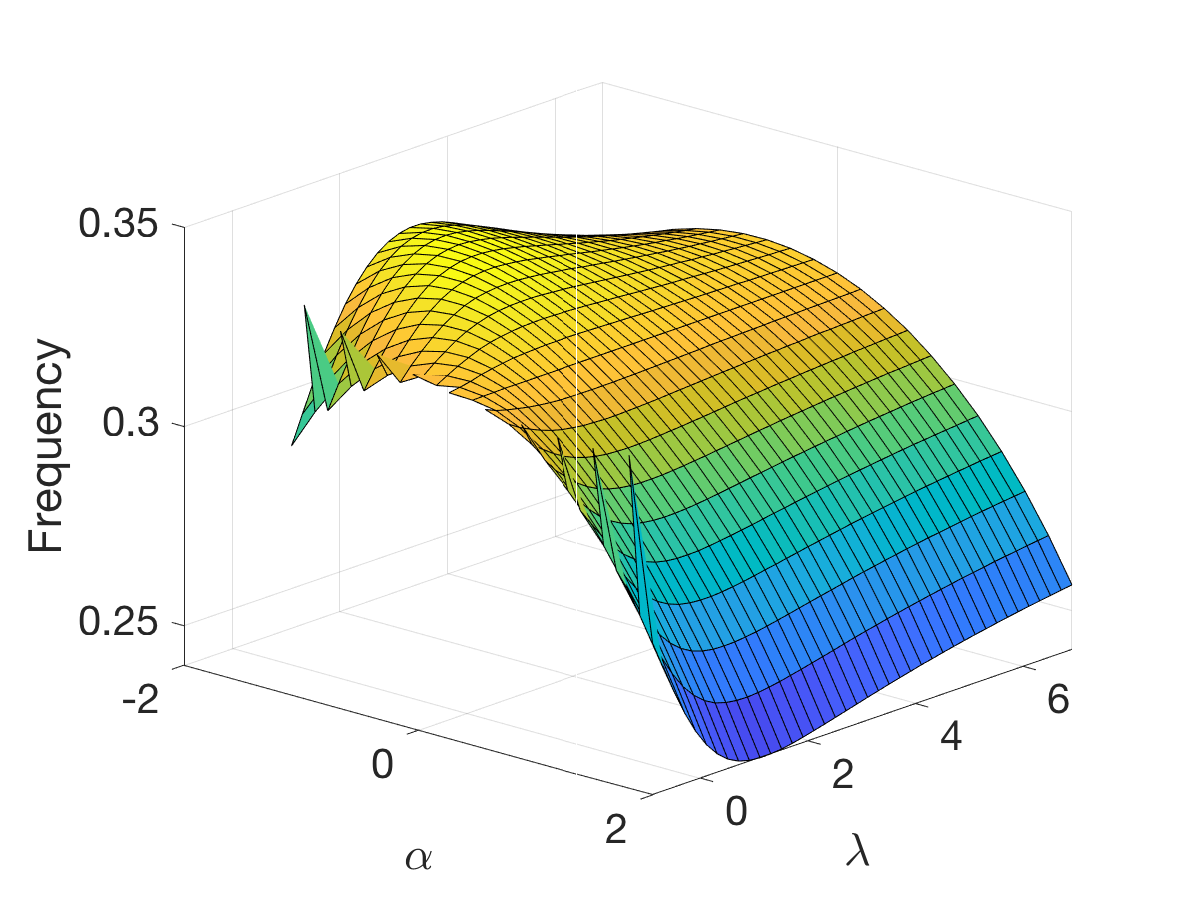
\includegraphics[width=1\linewidth]{Images/photo12_2.eps} 
  \end{minipage} 
 
  \caption{\textbf{Network frequency is not constant on amplitude LSs on the $\lambda-\alpha-b$ parameter space.} Left: amplitude LS ($A_{Net} = 1$) on the $\lambda-\alpha-b$ parameter space. Right: network frequency for each point on the amplitude LS. Parameter values: $a = 1$ and $\omega = 1$.}
  \label{photo12}
\end{figure}

We note that 1-dimensional total-degenerated LSs could be found in the $\lambda-\alpha-b$ parameter space following trajectories within the amplitude LS which preserve the network frequency.

\subsection{The $\omega-a$ parameter space}
If the $\omega-a$ parameter space is considered, similar results are obtained. More specifically, individual total-degenerated LSs on the $\omega-a$ parameter space are no longer total-degenerated in the self-connected cell due to the fact that frequency LSs do not preserve the network amplitude.

\begin{Statement}
Frequency level sets on the $\omega-a$ parameter space in the self-connected cell are not total-degenerated. The network amplitude is not preserved along frequency level sets on the $\omega-a$ parameter space.
\end{Statement}

Fig. (\ref{photo13}) shows a representative frequency LS ($f_{\text{Net}} = \pi^{-1}$) on the $\omega-\alpha-a$ parameter space. It is also shown the network amplitude for each point on the amplitude LS. 

\begin{figure}[h]
\centering
  \begin{minipage}{0.45\linewidth}
  \centering
    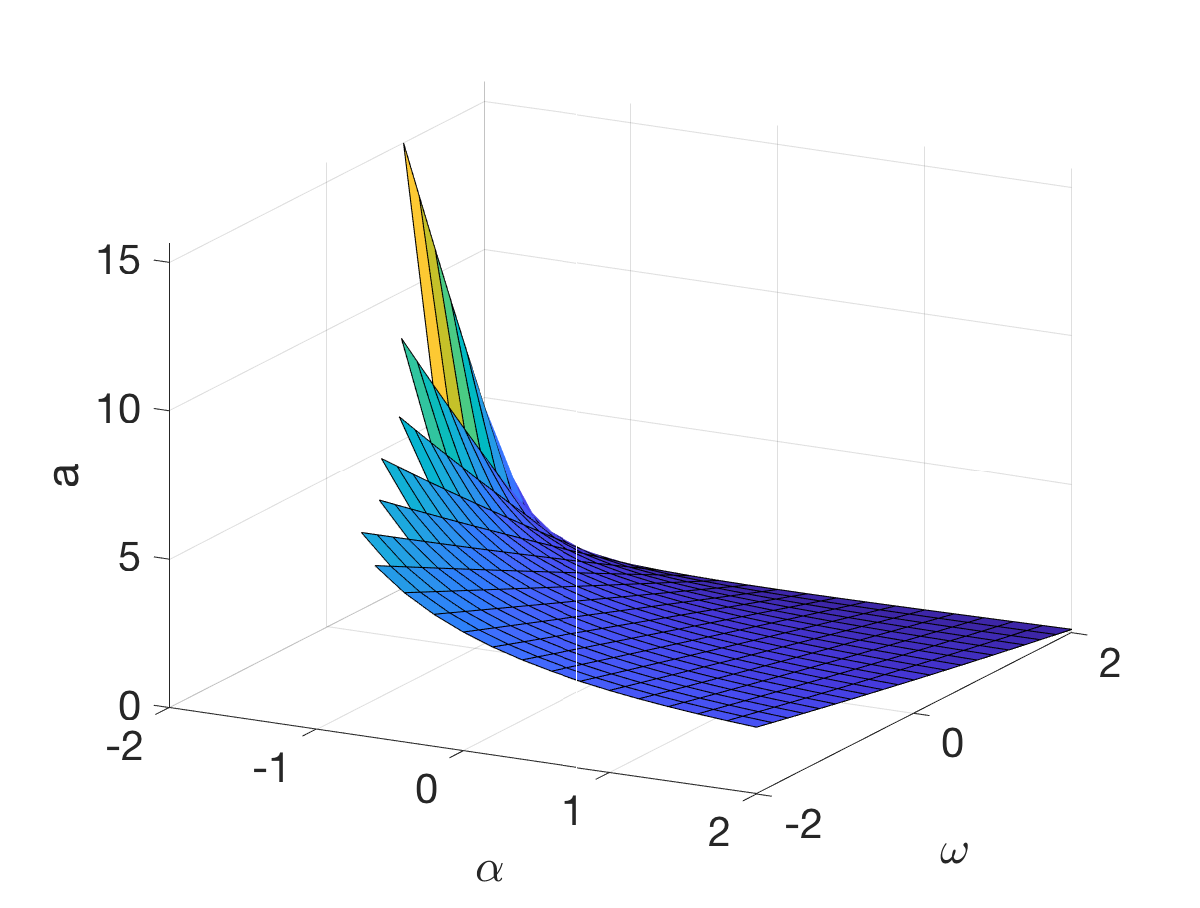
\includegraphics[width=1\linewidth]{Images/photo13_1.eps} 
  \end{minipage} 
  \begin{minipage}{0.45\linewidth}
  \centering
    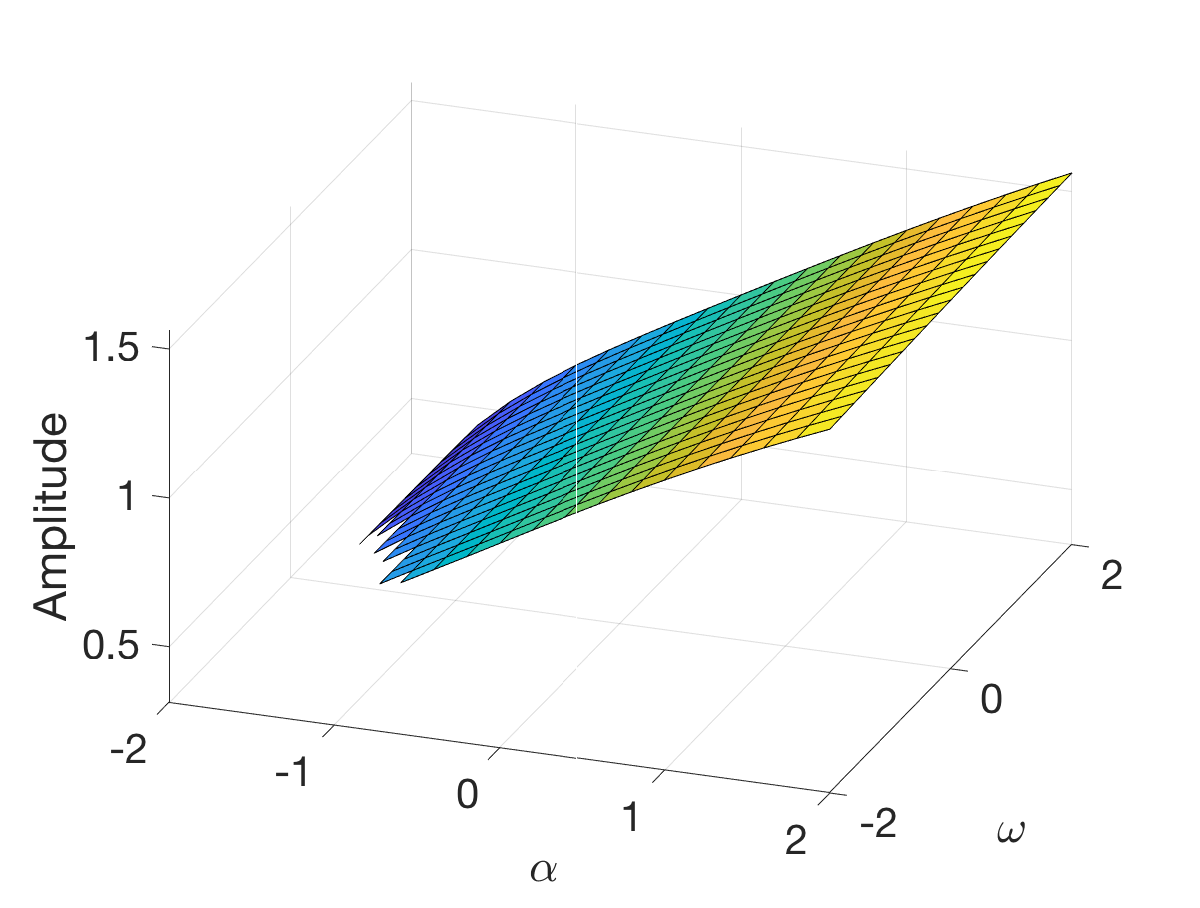
\includegraphics[width=1\linewidth]{Images/photo13_2.eps} 
  \end{minipage} 
 
 \caption{\textbf{Network amplitude is not constant on frequency LSs on the $\omega-\alpha-a$ parameter space.} Left: frequency LS ($A_{Net} = \pi^{-1}$) on the $\omega-\alpha-a$ parameter space. Right: network amplitude for each point on the frequency LS. Parameter values: $\lambda= 1$ and $b = 1$.}
  \label{photo13}
\end{figure}

We note that if the self-connectivity parameter $\alpha$ is fixed, amplitude does not remain constant on frequency LSs in the $\omega-a$ parameter space. Although it is indeed not constant, the variation in the network amplitude is quite small (not easily deduced from Fig. (\ref{photo13})-Right). As a consequence, the network amplitude does depend on parameters $\omega$ and $a$ in the self-connected cell, which is a new feature characterizing self-connected cells.

Furthermore, 1-dimensional total-degenerated LSs could be found in the $\omega-\alpha-a$ parameter space following trajectories within the frequency LS which preserve the network amplitude.

As a global picture, Fig. (\ref{photo14}) shows amplitude and frequency LSs in the form of colored heat graphs, where each point represents a single self-connected cell with a specific combination of parameters $\lambda$ and $b$ (top) and $\omega$ and $a$ (bottom) whose network amplitude (left) and frequency (right) corresponds with the value indicated on the color bar. LSs corresponds to the curves joining points with the same attribute value.

\begin{figure}[h]
\centering
\begin{minipage}{0.45\linewidth}
  \begin{center}
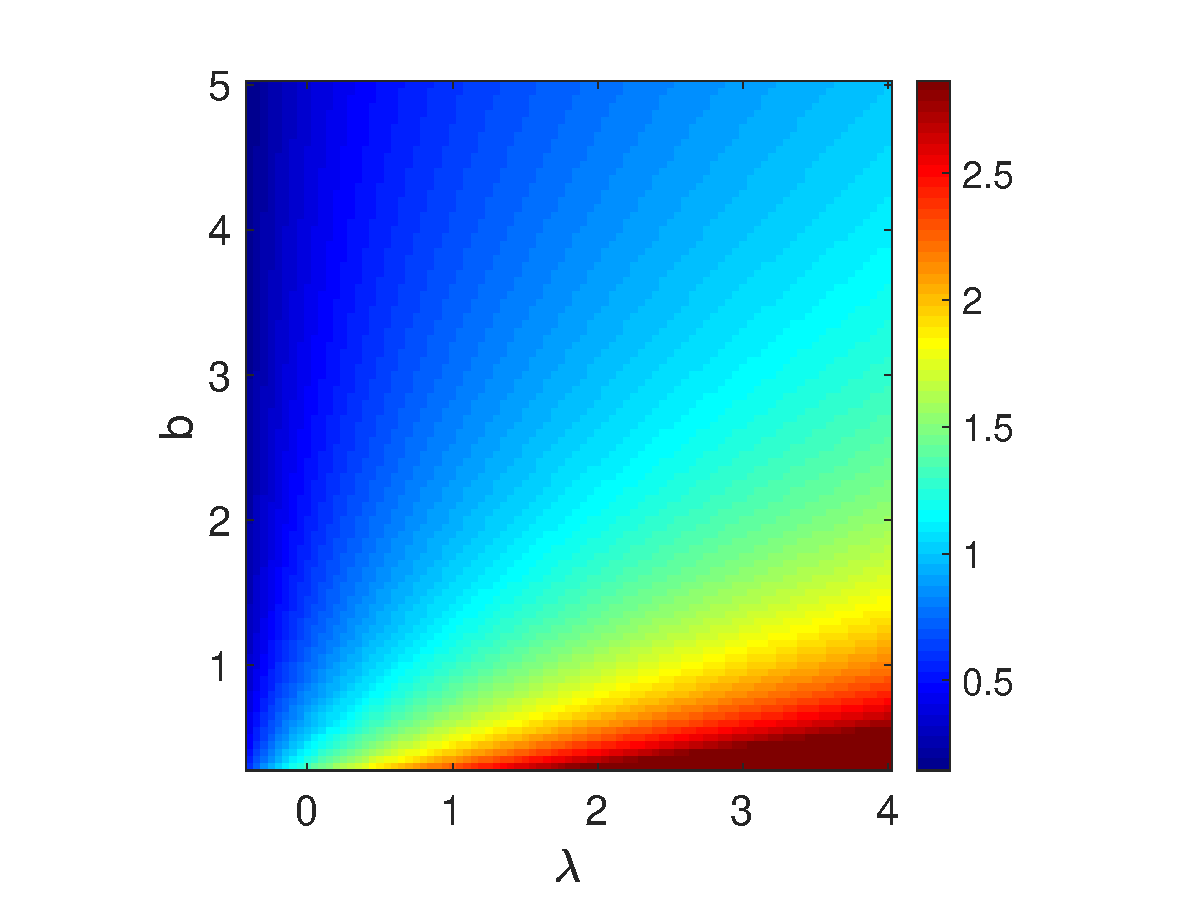
\includegraphics[width=1\linewidth]{Images/photo14_1.eps}
\end{center}
  \end{minipage} 
  \begin{minipage}{0.45\linewidth}
  \begin{center}
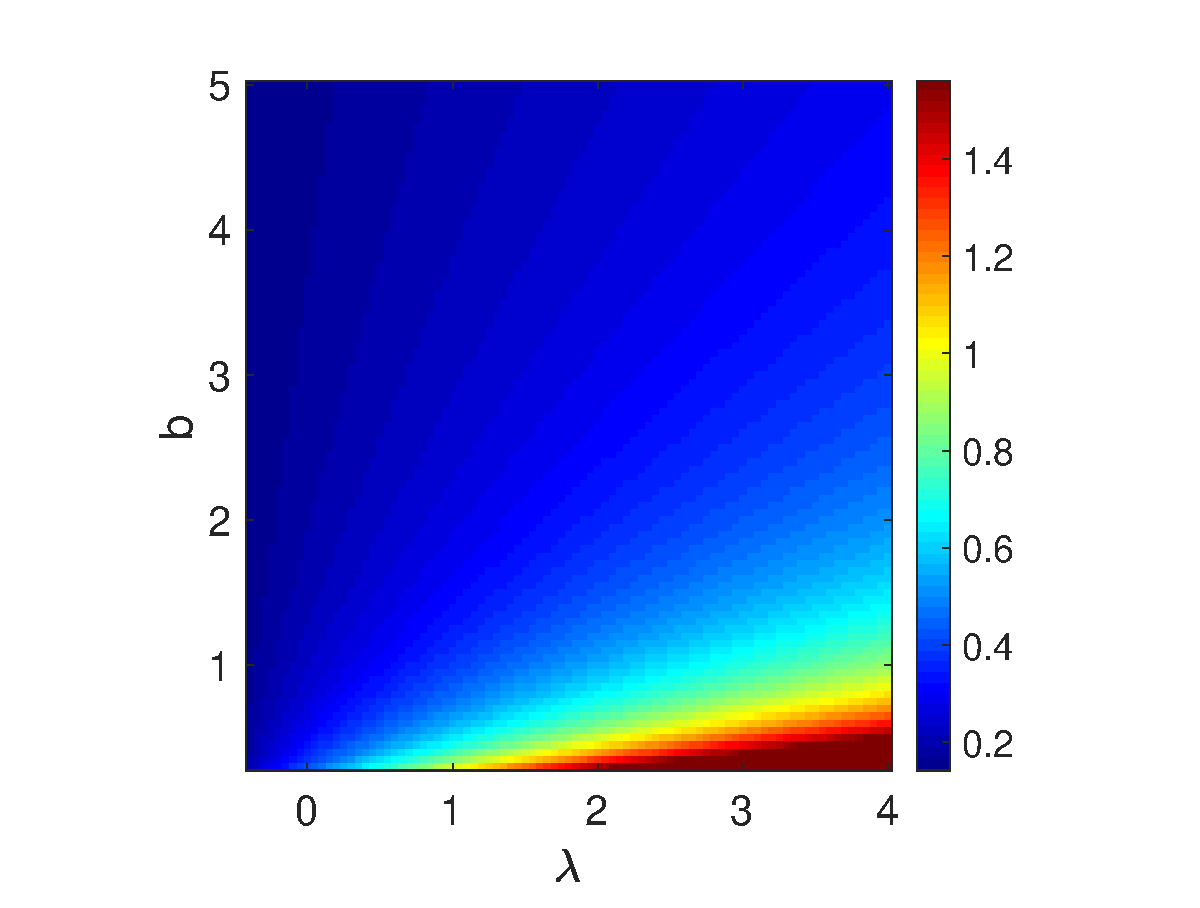
\includegraphics[width=1\linewidth]{Images/photo14_2.eps}
\end{center}

  \end{minipage} 
  
  \begin{minipage}{0.45\linewidth}
  \begin{center}
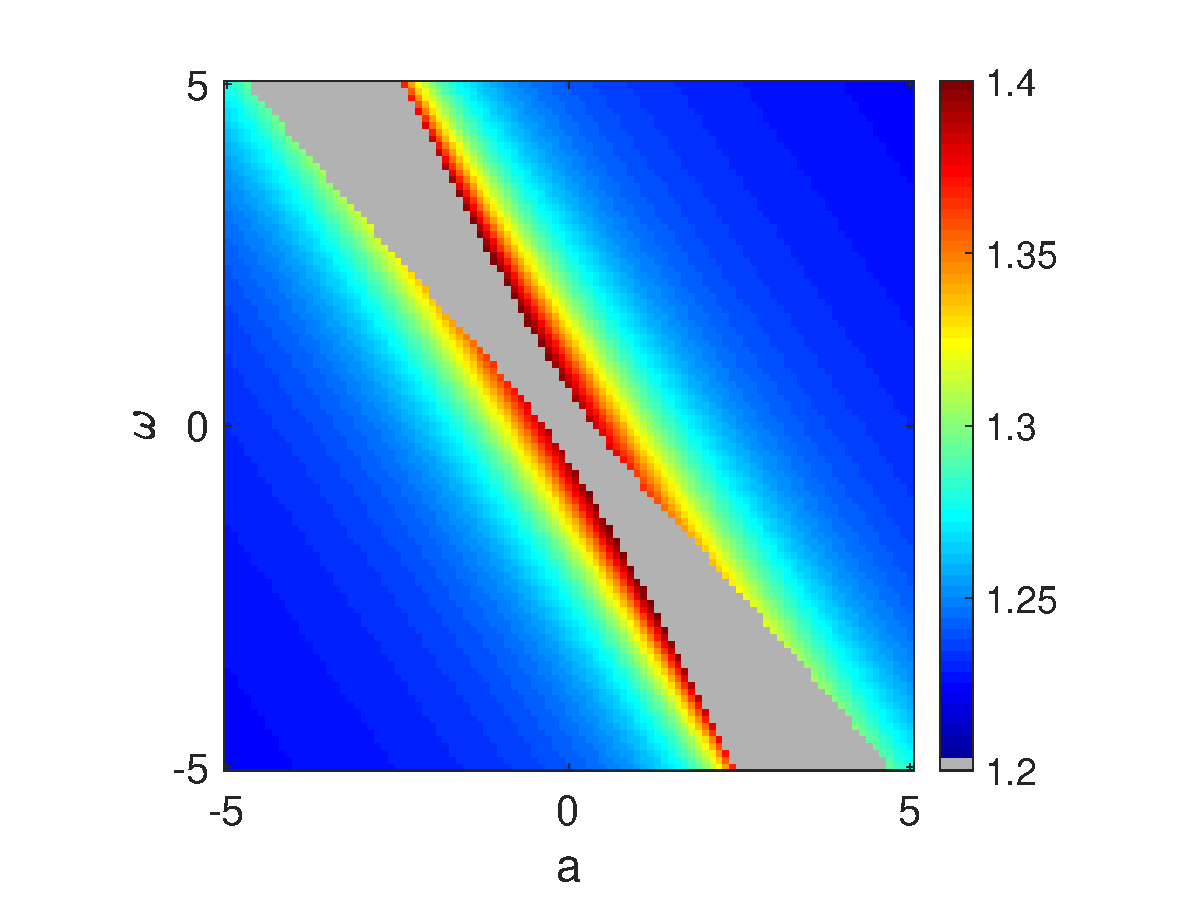
\includegraphics[width=1\linewidth]{Images/photo14_3.eps}
\end{center}
  \end{minipage} 
  \begin{minipage}{0.45\linewidth}
  \begin{center}
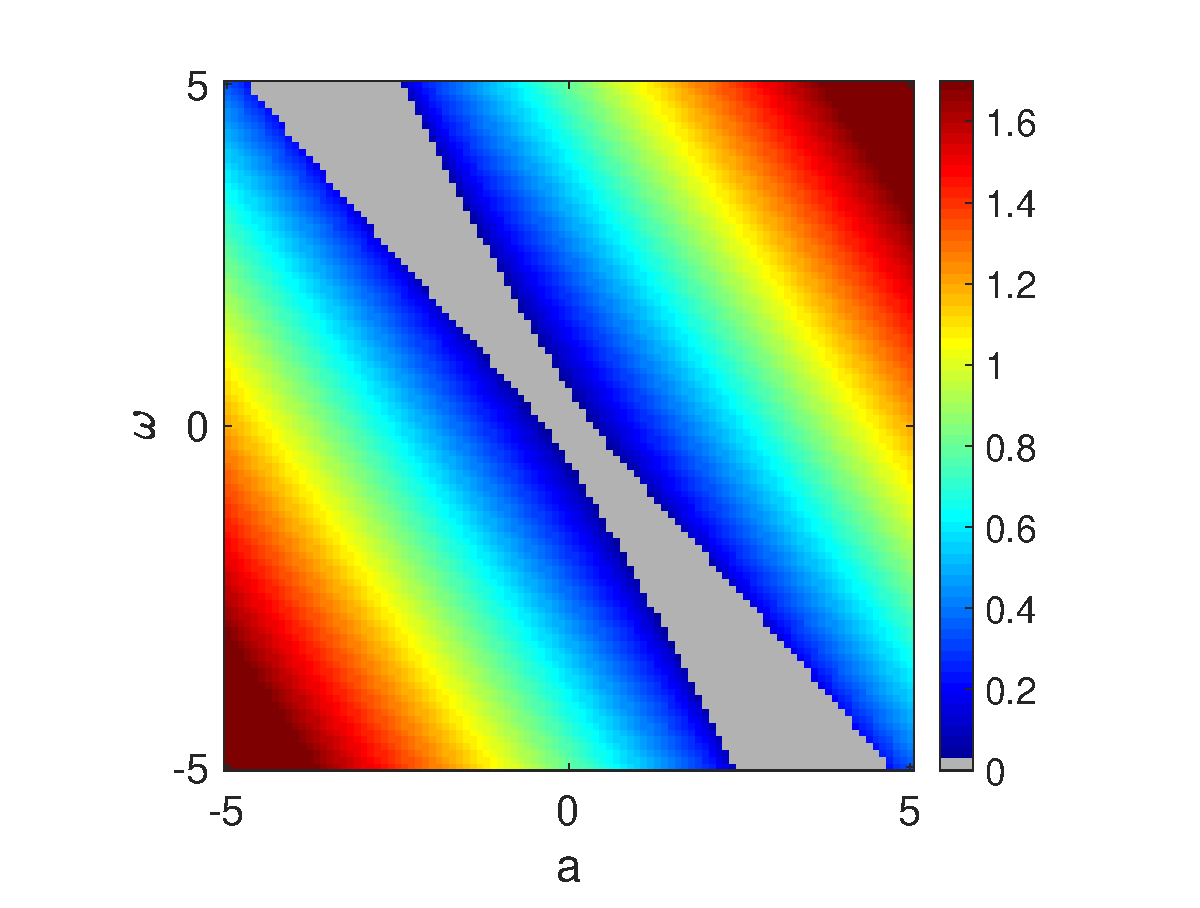
\includegraphics[width=1\linewidth]{Images/photo14_4.eps}
\end{center}

  \end{minipage} 
  
  \caption{\textbf{Amplitude and frequency LSs on the $\lambda-b$ and $\omega-a$ parameter spaces in the self-connected cell.} Top: amplitude (left) and frequency (right) LSs on the $\lambda-b$ parameter space. Bottom: amplitude (left) and frequency (right) LSs on the $\omega-a$ parameter space. The grey region corresponds to points in the parameter space for which there are not sustained oscillations. Parameter values. Top: $a = 1$, $\omega = 1$ and $\alpha = 1$. Bottom $\lambda = 1$, $b=1$ and $\alpha = 1$.}
  \label{photo14}
\end{figure}

\subsection{The whole intrinsic parameter space}
Once characterized amplitude and frequency LSs on the $\lambda-b$ and $\omega-a$ parameter spaces separately, we extent the parameter space in order to characterize total-degenerated LSs on the whole intrinsic parameter space.

We found 2-dimensional manifolds on the intrinsic parameter space preserving the network amplitude and frequency.

\begin{Statement}
The self-connected cell show 2-dimensional total-degenerated level sets on the intrinsic parameter space (the $a-b-\lambda-\omega$ parameter space).
\label{s10}
\end{Statement}

Computationally, we have found that in order to compute most general total-degenerated LSs, compensating parameters must be chosen appropriately. One of them must be either parameter $\lambda$ or $b$, whereas the other must be either parameter $\omega$ or $a$. This ensures that the most general total-degenerated LSs can be found.
 
Fig. (\ref{photo15}) shows an example of a total-degenerated LS ($A_{\text{Net}} = 1 $ and $f_{\text{Net}} = \pi^{-1}$) on the $a-b-\lambda-\omega$ parameter space in the self-connected cell for representative parameter values. In this case, we choose compensating parameters to be parameters $a$ and $b$. It shows in the form of colored heat graphs, compensated parameters $\lambda$ (left) and $\omega$ (right) for each pair of compensating parameters $a$ and $b$. Each point on the 2-dimensional manifold represents a self-connected cell with the same network amplitude ($A_{\text{Net}} = 1 $) and frequency ($f_{\text{Net}} = \pi^{-1}$).

  \begin{figure}[h]
  \centering
        \begin{minipage}{0.4\linewidth}
            \begin{center}
                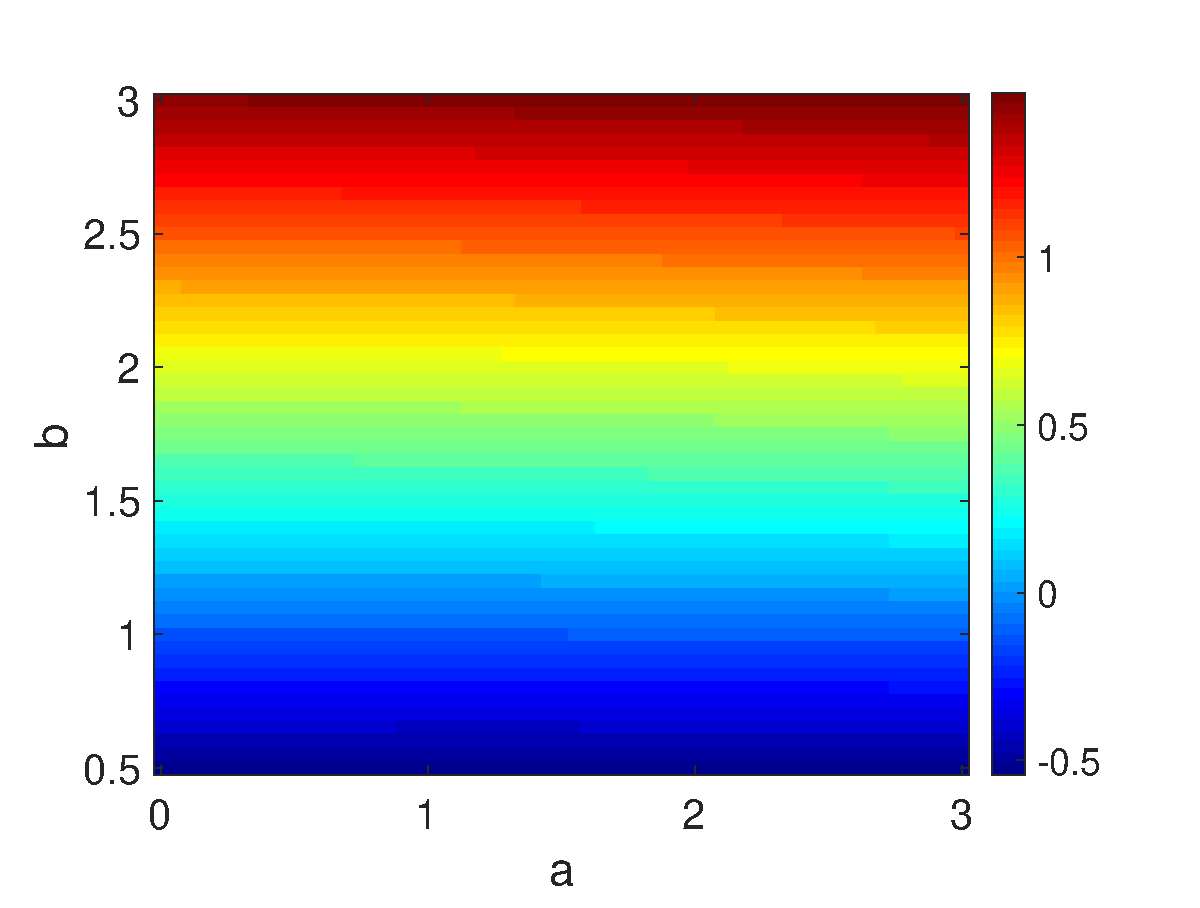
\includegraphics[width=1\linewidth]{Images/photo15_1.eps}
            \end{center}
        \end{minipage} 
        \begin{minipage}{0.4\linewidth}
            \begin{center}
                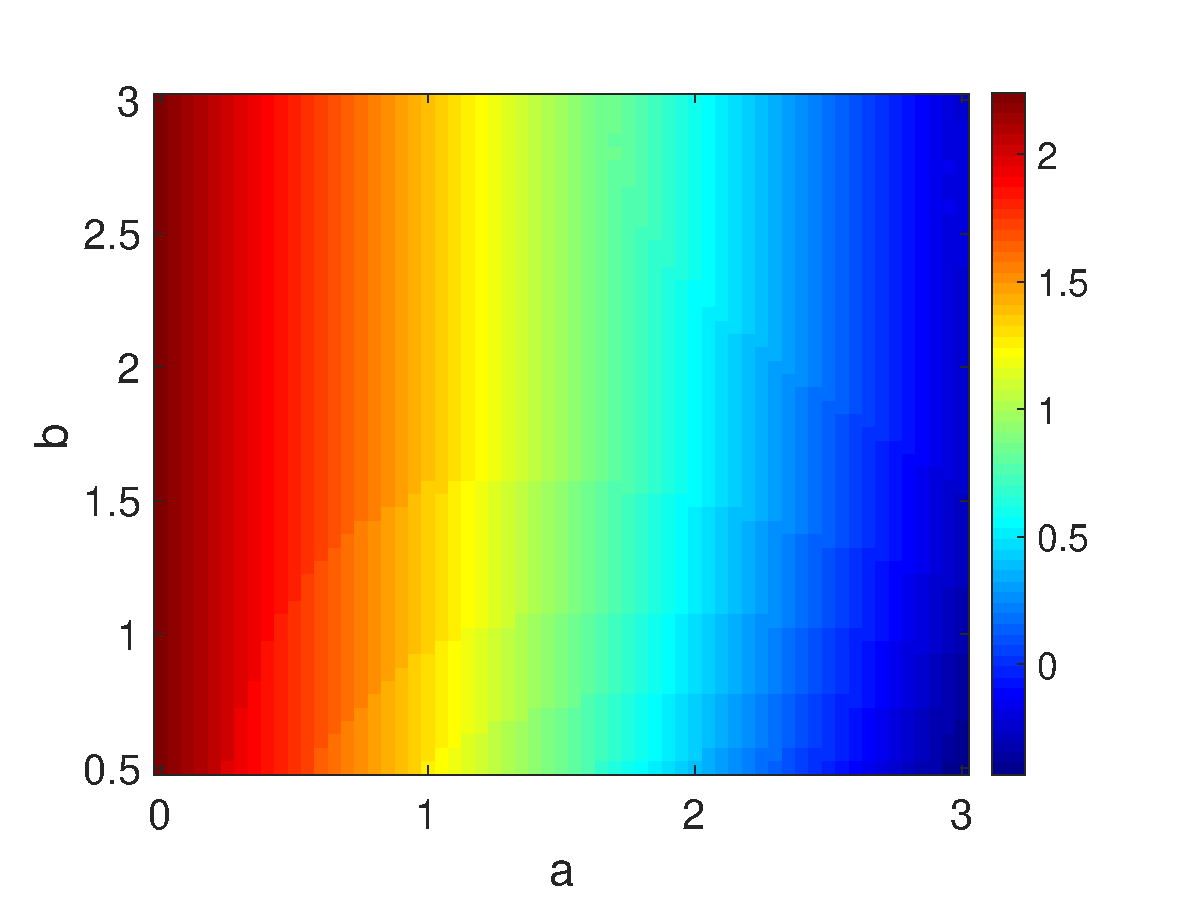
\includegraphics[width=1\linewidth]{Images/photo15_2.eps}
            \end{center}
        \end{minipage} 
  
  \caption{\textbf{Total-degenerated LS on the whole intrinsic parameter space in the self-connected cell.} The cell oscillates with amplitude $A_{\text{Net}} = 1$ and frequency $f_{\text{Net}} = \pi^{-1}$. For each pair of parameters $a$ and $b$, there are the values of parameters $\lambda$ (Left) and $\omega$ (Right), such as the amplitude and the frequency of the self-connected cell is preserved. Parameter values: $\alpha = 2$.}
  \label{photo15}
\end{figure}

Although individual total-degenerated LSs are also 2-dimensional manifolds on parameter space, there are some differences regarding compensatory functions, between total-degenerated LSs in the individual and the self-connected cell.

On the one hand, compensatory functions for total-degenerated LSs in the individual cell only depend on one compensating parameter. More specifically, parameter $b$ compensates parameter $\lambda$, while parameter $a$ compensates parameter $\omega$. 

On the other hand, compensatory functions in the self-connected cell depend on both compensating parameters, and therefore, each parameter ($\lambda$ and $\omega$) is compensated by both compensating parameters ($a$ and $b$).

In particular, Fig. (\ref{photo15}) shows the dependence on compensating parameters of compensatory functions on a representative total-degenerated LS ($A_{Net}=1$ and $f_{Net} = \pi^{-1}$). In order to gain insight into these compensatory dependencies between intrinsic parameters, we fix one compensating parameter and compute exact total-degenerated LS on the remaining 3-dimensional parameter space.

Fig. (\ref{photo16})-Left shows a representative total-degenerated LS on the $a-\lambda-\omega$ parameter space in which compensating parameter $b$ has been fixed. Conversely, Fig. (\ref{photo16})-Right shows a representative total-degenerated LS on the $b-\lambda-\omega$ parameter space in which compensating parameter $a$ has been fixed. 

  \begin{figure}[h]
  \centering
        \begin{minipage}{0.45\linewidth}
            \begin{center}
                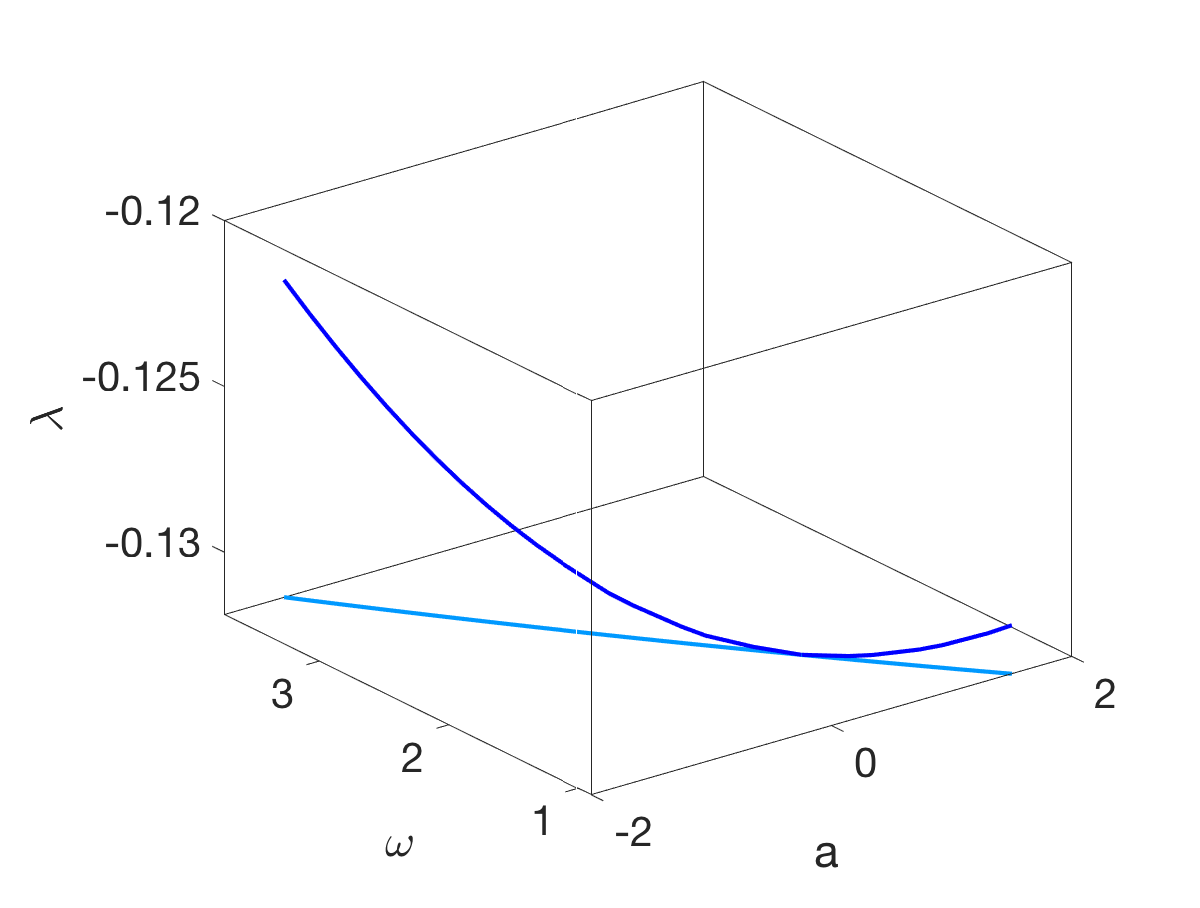
\includegraphics[width=1\linewidth]{Images/photo16_1.eps}
            \end{center}
        \end{minipage} 
        \begin{minipage}{0.45\linewidth}
            \begin{center}
                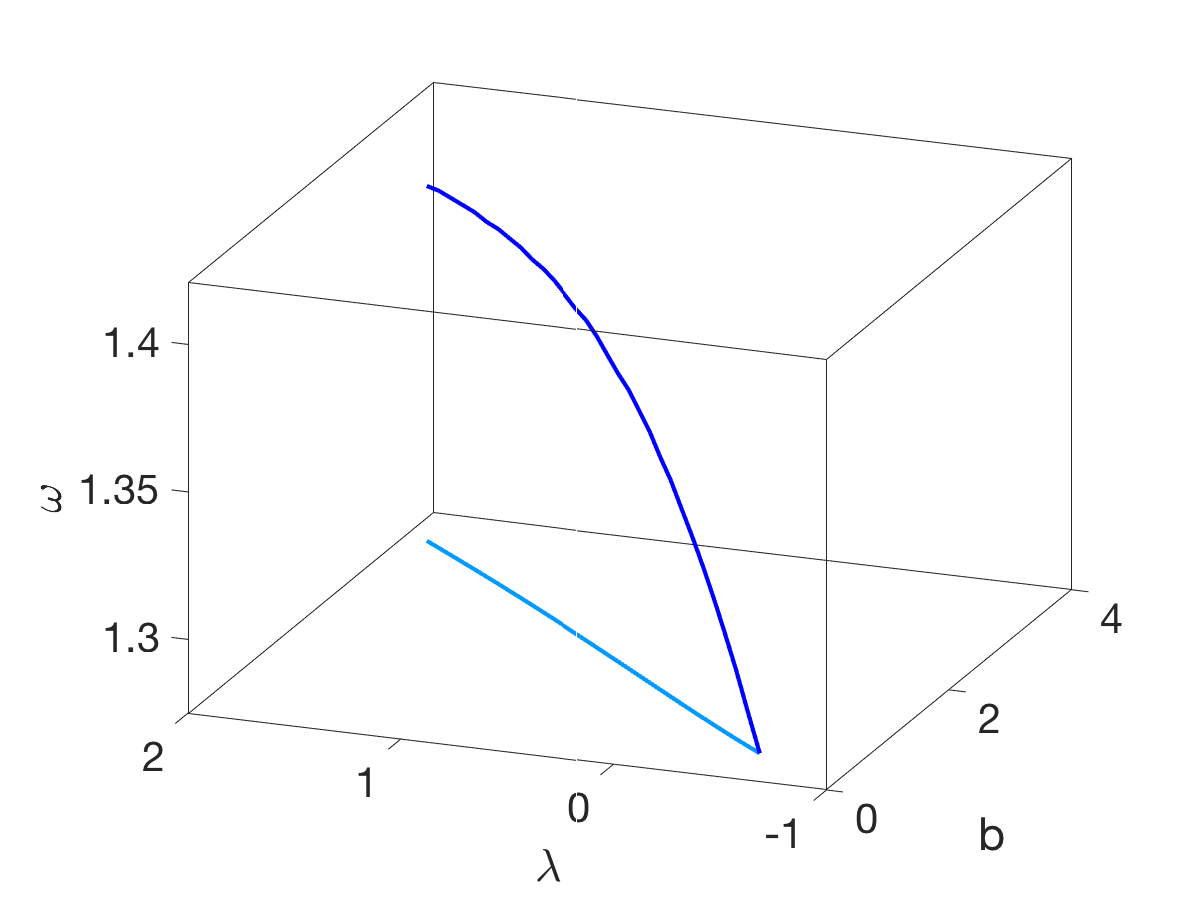
\includegraphics[width=1\linewidth]{Images/photo16_2.eps}
            \end{center}
        \end{minipage} 
  
  \caption{\textbf{Total-degenerated levels set on 3-dimensional intrinsic parameter spaces.} Left: compensating parameter $b$ is fixed and the 1-dimensional total-degenerated LS on the $a-\lambda-\omega$ parameter space is shown. Parameter values: $b=1$ and $\alpha=2$. Right: Compensating parameter $a$ is fixed and the 1-dimensional total-degenerated LS $a-\lambda-\omega$ parameter space is shown. Parameter values: $a=1$ and $\alpha=2$. Dark blue: 1-dimensional total-degenerated LSs. Light blue: LSs projections into $\omega-a$ (Left) and $\lambda-b$ (Right) parameter spaces.}
  \label{photo16}
\end{figure}

We see a monotonic and almost linear compensating dependencies between parameters $a-\omega$ and $b-\lambda$ in each case, which is clearly shown on the projection of each LS onto the $a-\omega$ or $b-\lambda$ parameter space (light blue lines in Fig. (\ref{photo16})). We note that the same type of compensating dependencies is observed in the individual cell.

In addition, parameters $\lambda$ (Fig. (\ref{photo16})-Left) and $\omega$ (Fig. (\ref{photo16})-Right) must be compensated in order to preserve network attributes. However, the strength of these new compensatory dependencies are weaker, since these additional compensated parameters are slightly changed, in comparison with parameters $\omega$ and $\lambda$, respectively.

The main reason of these parameter dependencies is the fact that the network frequency is mainly determined by parameters $\omega$ and $a$ and the network amplitude by parameters $\lambda$ and $b$. Therefore, although the self connection introduces new dependencies on parameters spaces $\lambda-b$ and $\omega-a$, these are weaker than the original ones.

\section{Homogeneous Two-Cell Networks}
In homogeneous two-cell networks, cells are identical and, therefore, they have same intrinsic parameters

\begin{equation}
   \lambda_{1}=\lambda_{2}(=\lambda) \text{,} \hspace{0.5cm} b_{1} = b_{2}(=b) \text{,} \hspace{0.5cm} a_{1}=a_{2}(=a) \hspace{0.5cm} \text{ and } \hspace{0.5cm} \omega_{1} = \omega_{2}(=\omega)
\end{equation}

\subsection{Symmetrical Networks}
\subsubsection{The connectivity parameter space}
In first place, we characterize amplitude and frequency LSs on the 4-dimensional connectivity parameter space in symmetrical homogeneous networks, where cells have the same network amplitude ($A_{\text{Net}}$) and frequency ($f_{\text{Net}}$) value.

Fig. (\ref{photo17}) shows an example of an amplitude LS ($A_{\text{Net}}=1.5$) on the connectivity parameter space for representative parameter values. It is also shown the network frequency ($f_{\text{Net}}$) for each point on the amplitude LS.

  \begin{figure}[h]
        \begin{minipage}{0.32\linewidth}
            \begin{center}
                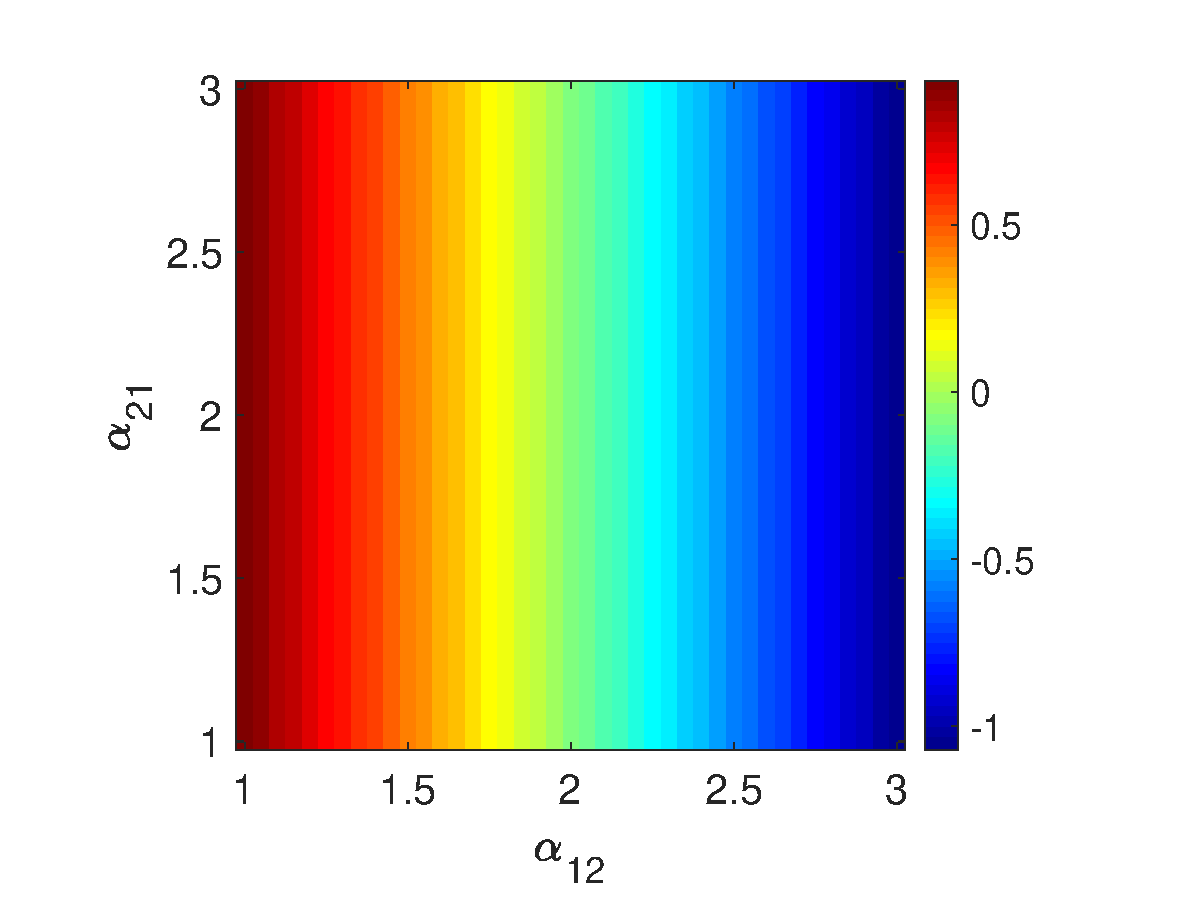
\includegraphics[width=1\linewidth]{Images/photo17_1.eps}
            \end{center}
        \end{minipage} 
        \begin{minipage}{0.32\linewidth}
            \begin{center}
                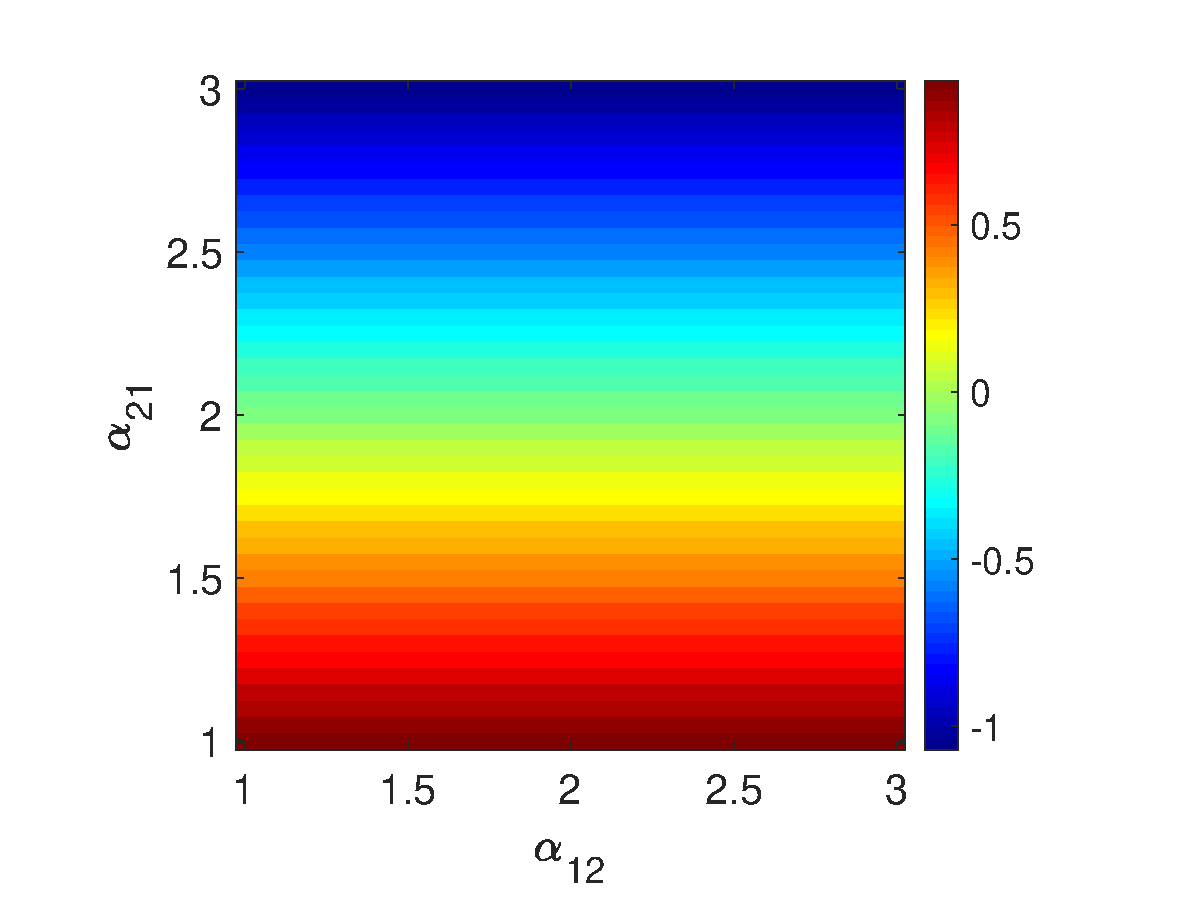
\includegraphics[width=1\linewidth]{Images/photo17_2.eps}
            \end{center}
        \end{minipage} 
    \begin{minipage}{0.32\linewidth}
        \begin{center}
            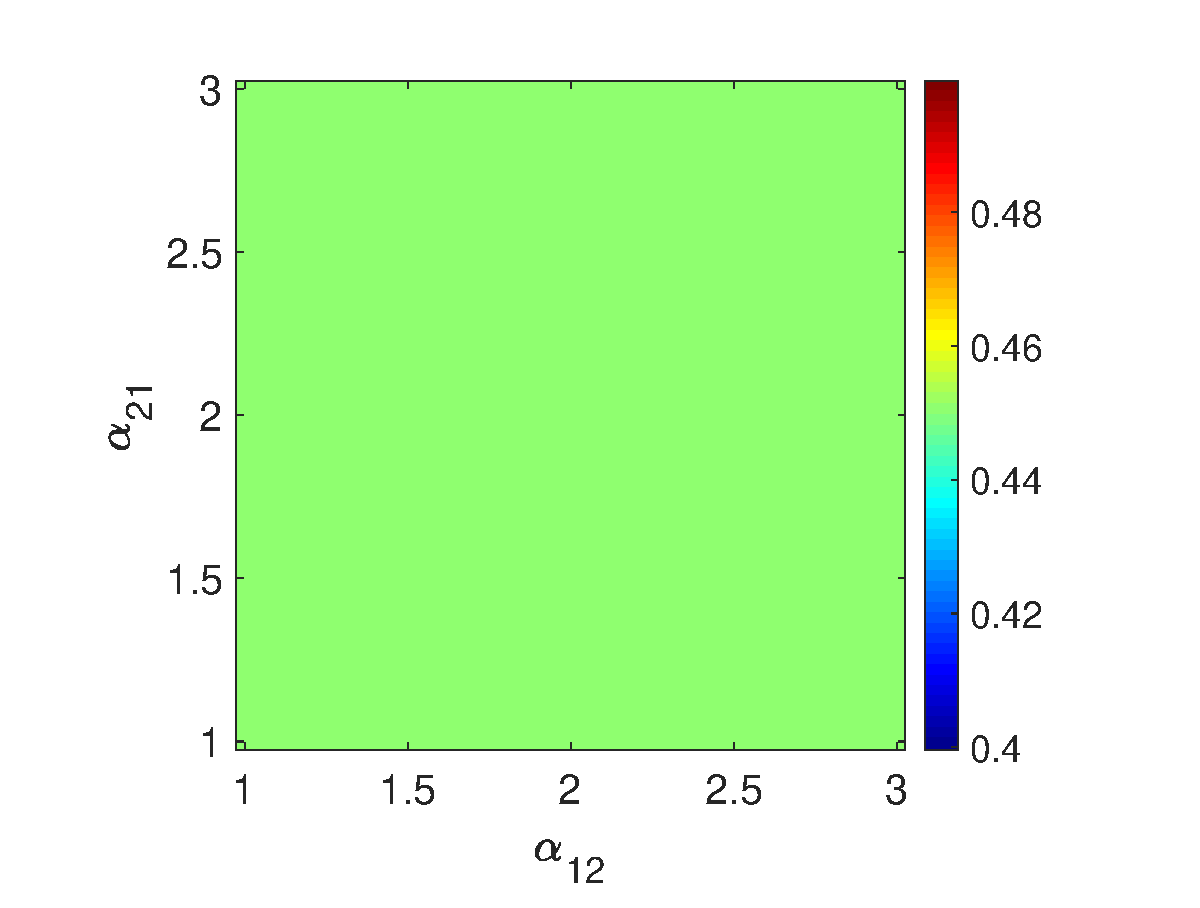
\includegraphics[width=1\linewidth]{Images/photo17_3.eps}
        \end{center}
    \end{minipage} 
  
  \caption{\textbf{Amplitude LS on the connectivity parameter space in symmetrical homogeneous two-cell networks.} Cell-1 and cell-2 oscillate with amplitude value 1.5. Left and middle: amplitude LS. For each pair of cross-connectivity parameters, there are the values of self-connectivity parameters, $\alpha_{11}$ (Left) and $\alpha_{22}$ (Middle), such as the network amplitude is preserved. Right: frequency for each point of the amplitude LS. Parameter values: $\lambda = 1$, $b=1$, $a = 1$, $\omega= 1$.}
  \label{photo17}
\end{figure}

The next statement summarizes the main features of amplitude and frequency LSs on the connectivity parameter space in symmetrical homogeneous two-cell networks.

\begin{Statement}
Symmetrical homogeneous networks show 2-dimensional amplitude level sets on the connectivity parameter space. Furthermore, the network frequency is constant throughout amplitude level sets on the connectivity parameter space. Consequently, symmetrical homogeneous networks show 2-dimensional total-degenerated level sets on the connectivity parameter space.
\end{Statement}

Symmetrical homogeneous networks are of interest because total-degenerated  LSs on the connectivity parameter space can be easily characterized. For a given pair of cross-connectivity parameter $\alpha_{12}$ and $\alpha_{21}$, compensated self-connectivity parameters $\alpha_{11}$ and $\alpha_{22}$ can be found in order to preserve a given network amplitude.

Fig (\ref{photo18}) shows how breaking the condition for LSs preservation in synchronized homogeneous networks, Eq. (\ref{e29}), affects individual amplitude and frequency LSs. Here, cross-connectivity parameter are fixed and self-connectivity parameters are perturbed from it LSs preserving value. Both self-connectivity parameters are perturbed the same amount so as to guarantee a symmetrical network. Top plots show the effect of mutually higher self-connectivity, whereas bottom plots shows the effect of mutually lower self-connectivity. 

\begin{figure}[h]
\centering
  \begin{minipage}{0.45\linewidth}
  \centering
    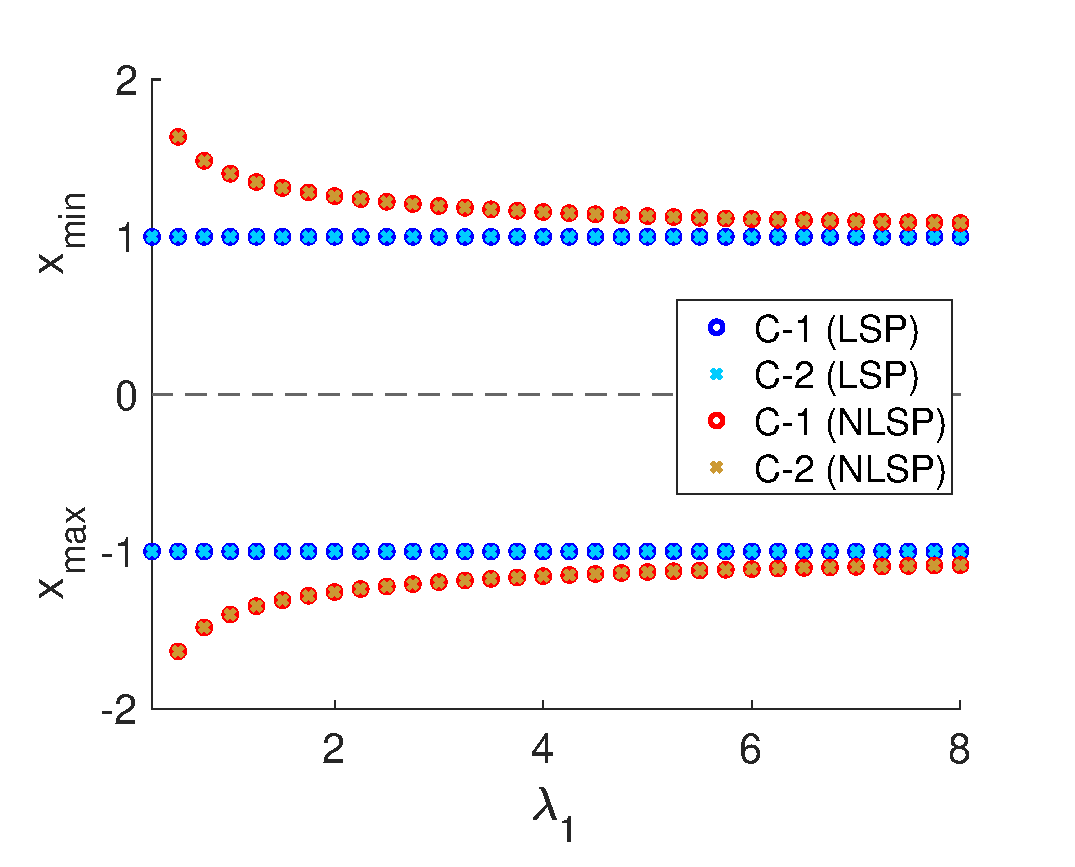
\includegraphics[width=1\linewidth]{Images/photo18_1.eps} 
  \end{minipage} 
  \begin{minipage}{0.45\linewidth}
  \centering
    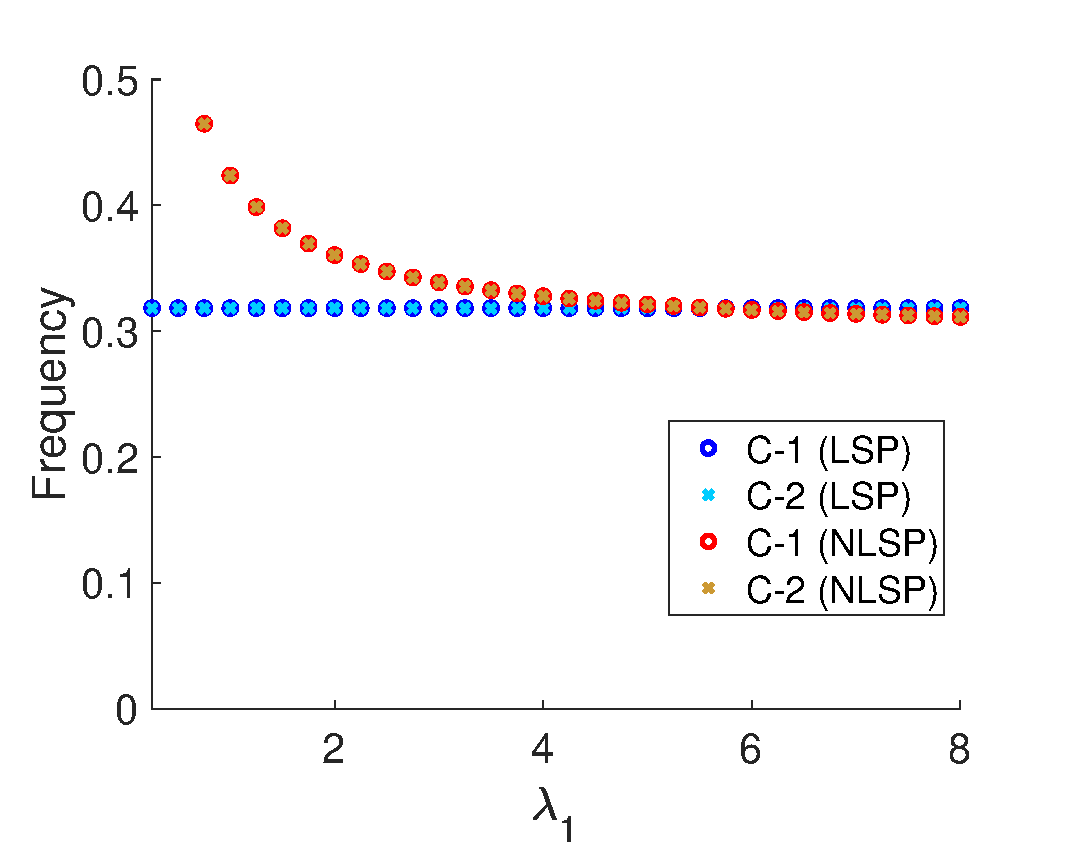
\includegraphics[width=1\linewidth]{Images/photo18_2.eps} 
  \end{minipage} 
  
  \begin{minipage}{0.45\linewidth}
  \centering
    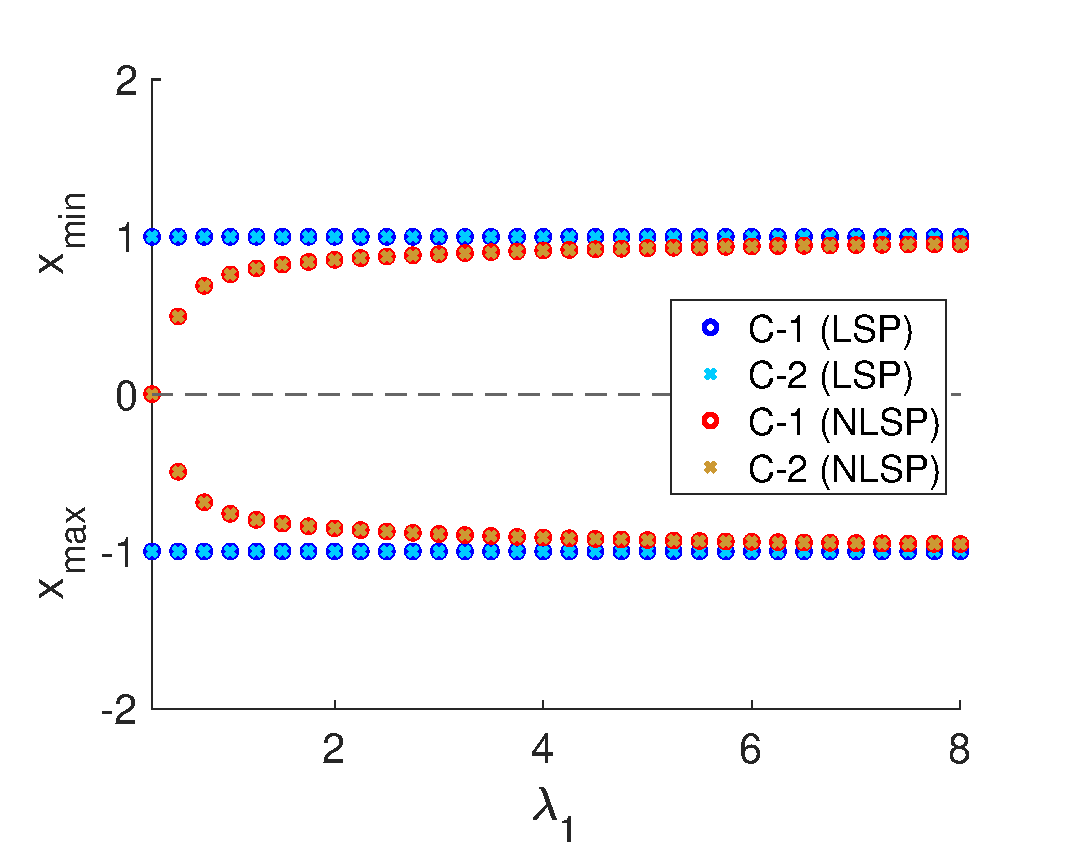
\includegraphics[width=1\linewidth]{Images/photo18_3.eps} 
  \end{minipage} 
  \begin{minipage}{0.45\linewidth}
  \centering
    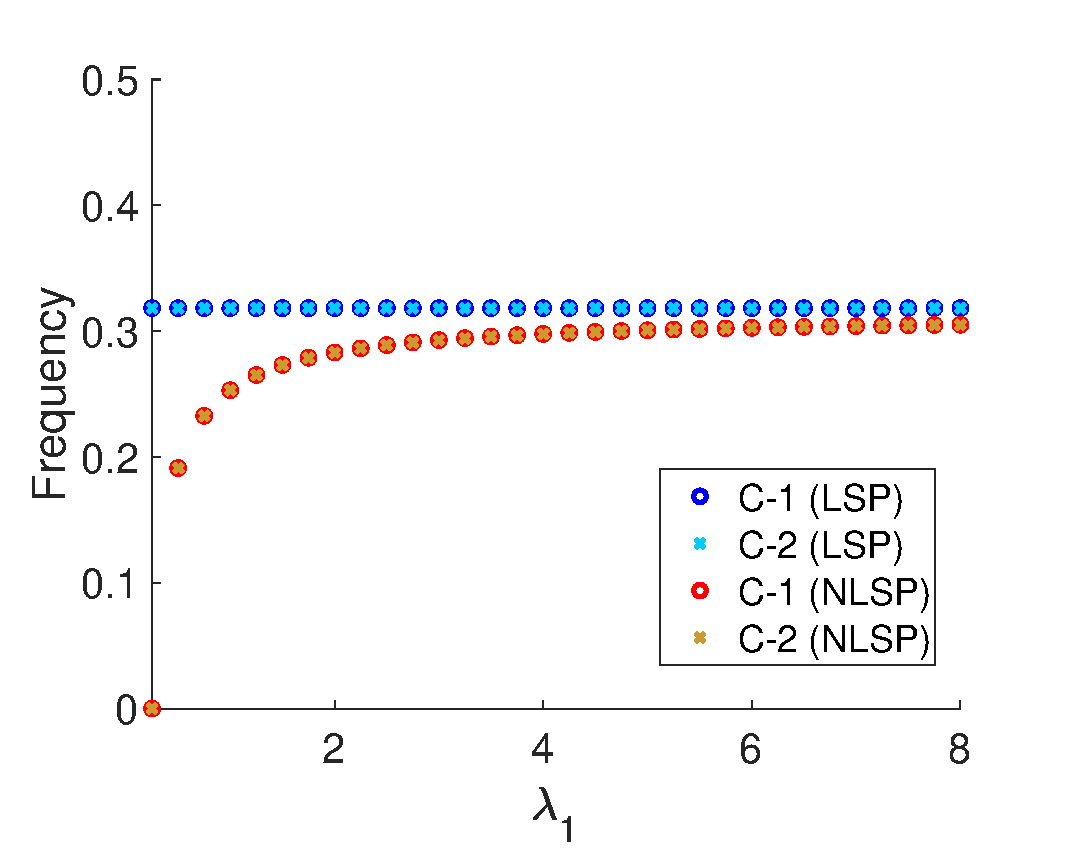
\includegraphics[width=1\linewidth]{Images/photo18_4.eps} 
  \end{minipage} 
  
    \caption{\textbf{Effect of mutually higher and lower self-connectivity (compared to the self-connectivity preserving individual LSs) on individual amplitude LSs in synchronized homogeneous networks.} Top: mutually higher self-connectivity. Parameter values: $a = 1$, $\omega = 1$, $\alpha_{12}=1$, $\alpha_{21}=1$, $\alpha_{11}=0.5$ and $\alpha_{22}=0.5$ (Perturbation: $+1.5$). Bottom: mutually lower self-connectivity. Parameter values: $a = 1$, $\omega = 1$, $\alpha_{12}=1$, $\alpha_{21}=1$, $\alpha_{11}=-1.75$ and $\alpha_{22}=-1.75$ (Perturbation $-0.75$). Left: amplitude  envelope  diagram  for values  $(\lambda,b)$  belonging  to the  same individual  amplitude  LS. Right: frequency  diagram  for  values  $(\lambda,b)$ belonging  to  the  same  individual  amplitude LS. LSP refers to the LS preserving network in which connectivity parameters preserve individual LSs. NLSP refers to perturbed networks in which self-connectivity parameters have been modified.}
  \label{photo18}
\end{figure}

In particular, we see that a mutual increase in self-connectivity leads to higher amplitude symmetrical networks, while a mutual decrease in self-connectivity produces symmetrical networks with lower amplitude values.

More specifically, for a given network amplitude value ($A_{\text{Net}}$), the network amplitude LS on connectivity parameter space is given by

\begin{equation}
    C_{A_{\text{Net}}} = 
    \begin{pmatrix}
        -\alpha_{12} + \varepsilon(A_{\text{Net}}) & \alpha_{12}\\
        \alpha_{21} & -\alpha_{21} + \varepsilon(A_{\text{Net}})
    \end{pmatrix}
    \text{ , } \hspace{0.5cm} \alpha_{12},\alpha_{21} \geq 0 \hspace{0.5cm} \text{or} \hspace{0.5cm}  \alpha_{12},\alpha_{21} \leq 0 
    \label{e37}
\end{equation}

where $\varepsilon(A_{\text{Net}})$ is a constant dependent on the network amplitude $A_{\text{Net}}$. Interestingly, the compensatory function associated with each self-connectivity parameter only depends on its corresponding cross-connectivity parameter. In other words, cross-connectivity parameter $\alpha_{12}$ only compensates self-connectivity parameter $\alpha_{11}$, while cross-connectivity parameter $\alpha_{21}$ only compensates self-connectivity parameter $\alpha_{22}$.

As it is expected, when the network amplitude equals the individual cell amplitude ($A_{Net} = A_{Ind}$), the network amplitude LS corresponds to the LS on the connectivity parameter space which preserve individual LSs, Eq. (\ref{e29}).

\subsubsection{Changing intrinsic parameters}
Since the network frequency ($f_{\text{Net}}$) is constant throughout amplitude LSs on the connectivity parameter space, there is a correspondence between a given network amplitude LS on connectivity parameter space and its frequency. If for a given network amplitude LS on connectivity parameter space, a different network frequency is required, intrinsic parameters must be changed. However, the network amplitude LS on connectivity parameter space might change. In other words, self-connectivity parameters might be differently compensated for a given pair of cross-connectivity parameters.

In Fig. (\ref{photo19}), we show the network frequency on the amplitude LS ($A_{\text{Net}} = 1.5$) on connectivity parameter space as a function of parameters $\lambda$ and $b$. We also compare the network frequency ($f_{\text{Net}}$) with the individual cell frequency ($f_{\text{Ind}}$).

\begin{figure}[h]
  \begin{minipage}{0.32\linewidth}
            \begin{center}
             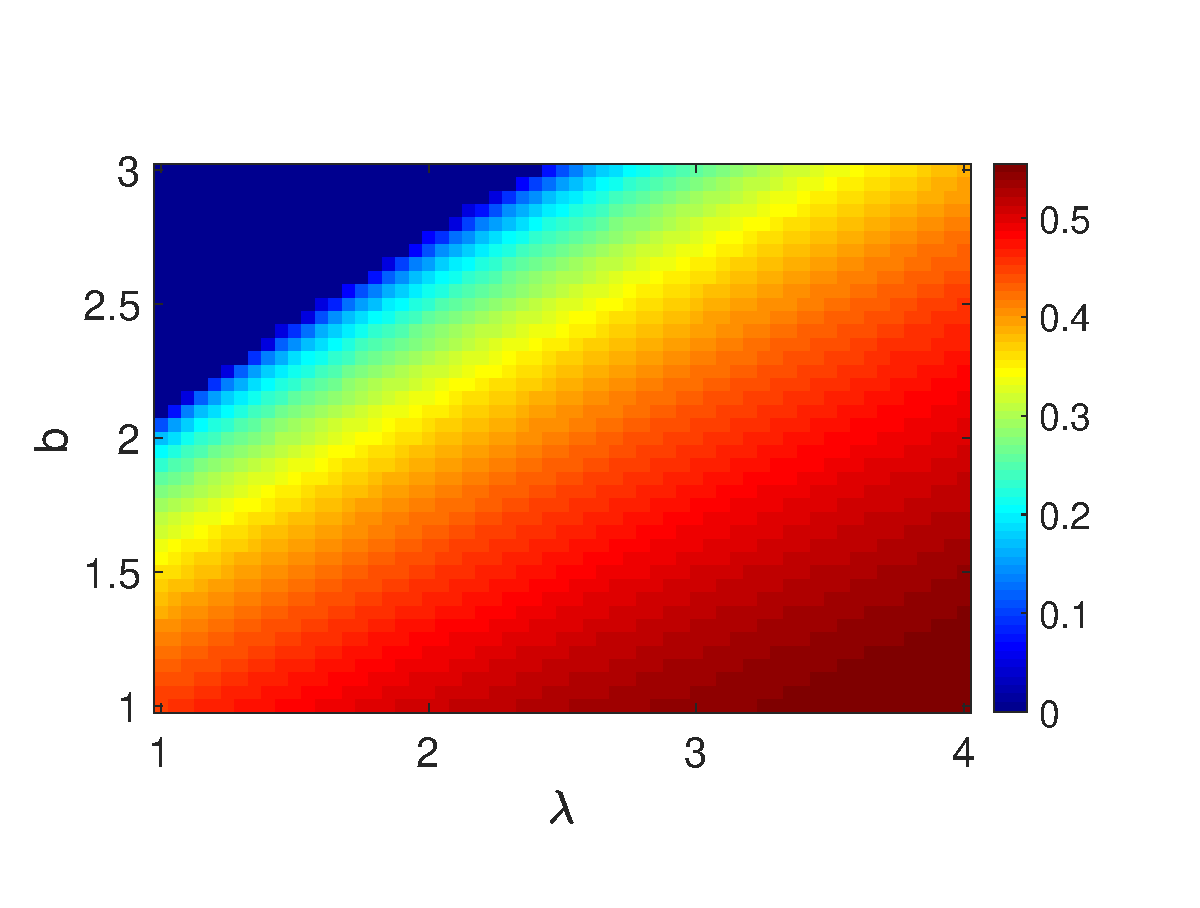
\includegraphics[width=1\linewidth]{Images/photo19_1.eps}
            \end{center}
        \end{minipage} 
        \begin{minipage}{0.32\linewidth}
            \begin{center}
                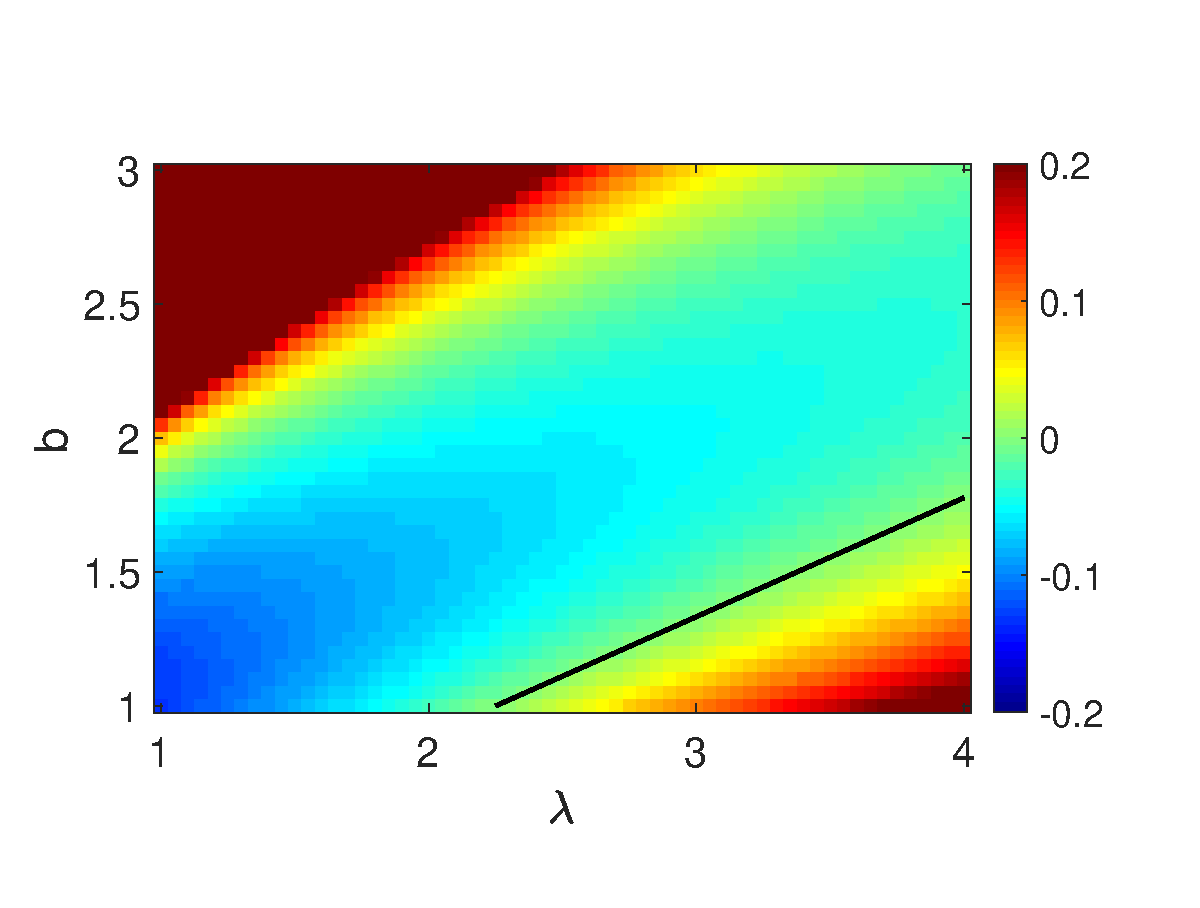
\includegraphics[width=1\linewidth]{Images/photo19_2.eps}
            \end{center}
        \end{minipage} 
        \begin{minipage}{0.32\linewidth}
            \begin{center}
                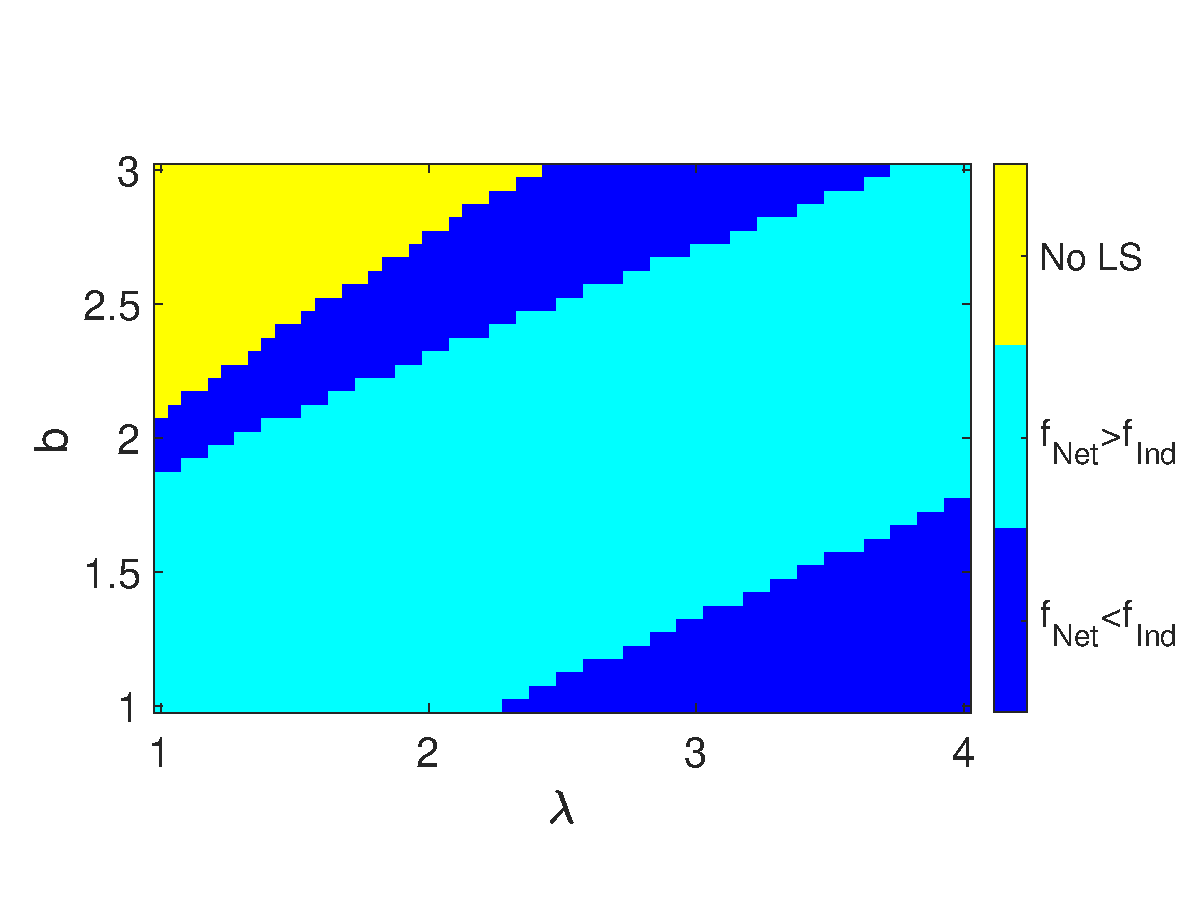
\includegraphics[width=1\linewidth]{Images/photo19_3.eps}
            \end{center}
        \end{minipage} 
  \caption{\textbf{Intrinsic parameters change the value of the network frequency preserved on a given amplitude LS on connectivity parameter space.} Both cells oscillate with amplitude value 1.5 ($A_{\text{Net}} = 1.5$). Left: network frequency on the amplitude LS ($A_{\text{Net}} = 1.5$) on connectivity parameter space as a function of parameters $\lambda$ and $b$. Middle: the difference between the individual cell frequency and the network frequency (from left). The blank line represents the case in which the individual LS ($K_{a}=2.25$ and $K_{f} = 3.25$) is preserved. Right: regions where the network frequency is higher or lower than the individual cell frequency (from Middle). Parameter values: $a = 1$, $\omega = 1$, $\alpha_{12} = 1$ and $\alpha_{21}=1$.}
  \label{photo19}
\end{figure}

Curves preserving the frequency in Fig. (\ref{photo19})-Left represent 1-dimensional total-degenerated LSs on the $\lambda-b-\alpha_{11}-\alpha_{22}$ parameter space. As an exception, black line in (\ref{photo19})-Middle is the only curve in which the value of self-connectivity parameters $\alpha_{11}$ and $\alpha_{22}$ does not change (same amplitude LS on connectivity parameter space). It corresponds to the case where individual LS are preserved in the two-cell network. 

\subsection{Non-symmetrical Networks}
In non-symmetrical homogeneous networks, the amplitude value of each cell on a given amplitude LS is different. Fig. (\ref{photo20}) shows an example of an amplitude LS ($A_{1} = 1.5$ and $A_{2}=1.25$) in a non-symmetrical homogeneous networks for representative parameter values. It is also shown the network frequency for each point in the amplitude LS.

\begin{figure}[h]
  \begin{minipage}{0.32\linewidth}
  \begin{center}
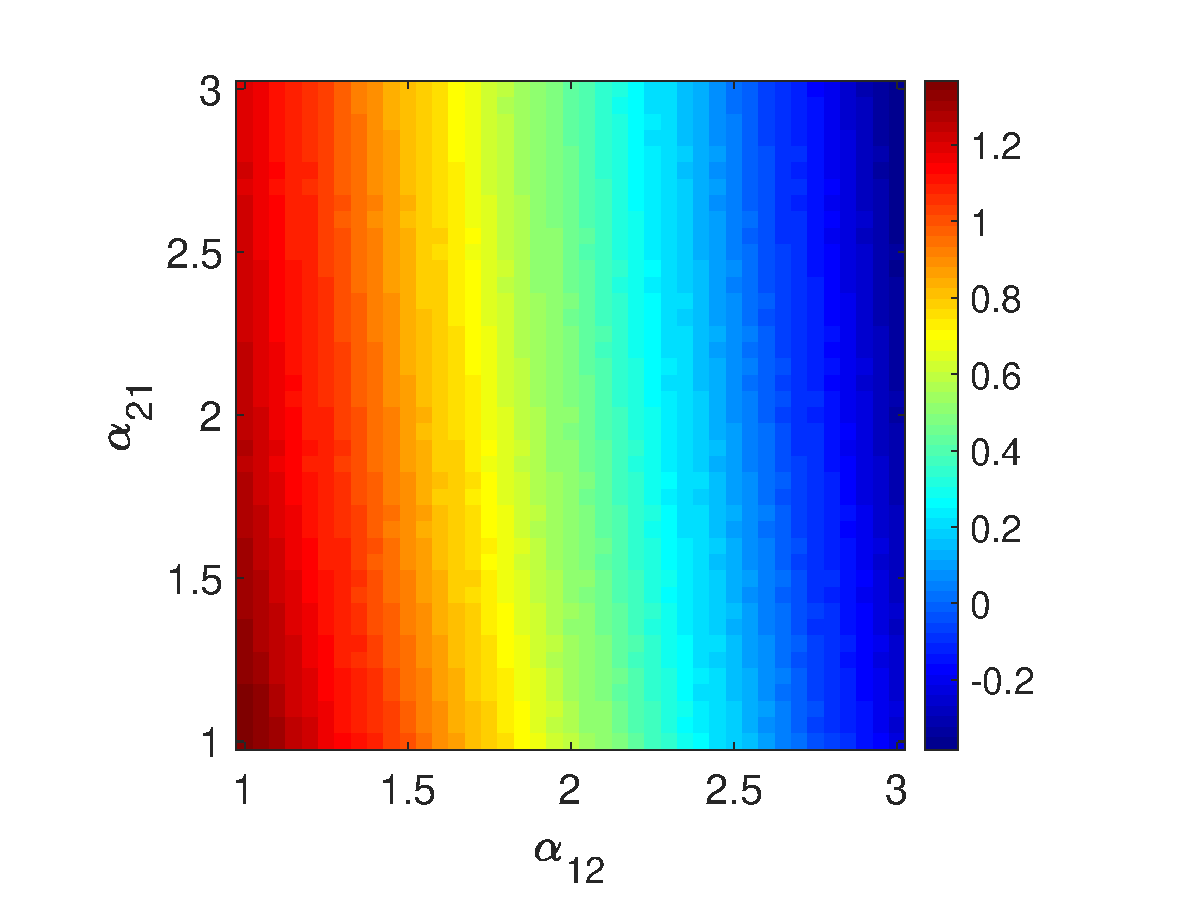
\includegraphics[width=1\linewidth]{Images/photo20_1.eps}
\end{center}
  \end{minipage} 
  \begin{minipage}{0.32\linewidth}
  \begin{center}
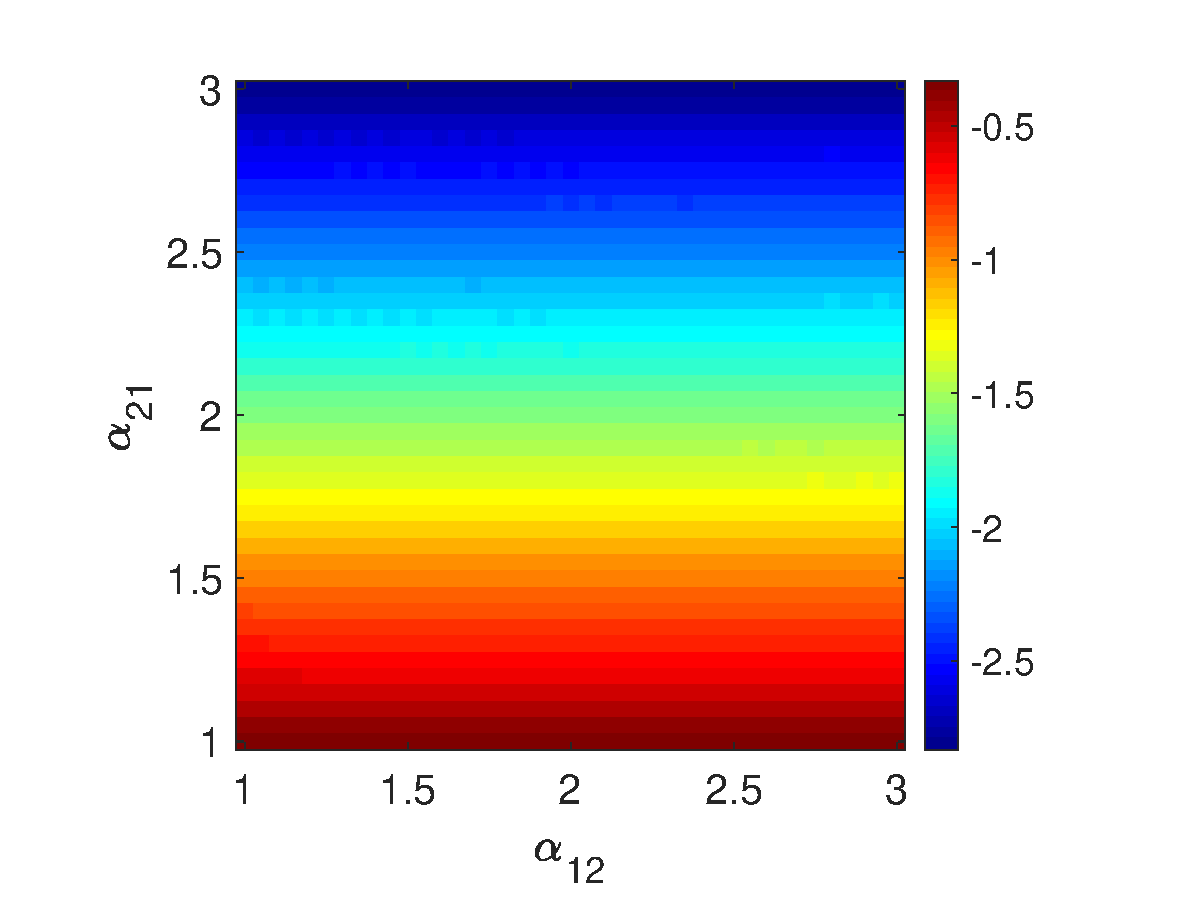
\includegraphics[width=1\linewidth]{Images/photo20_2.eps}
\end{center}

  \end{minipage} 
   \begin{minipage}{0.32\linewidth}
  \begin{center}
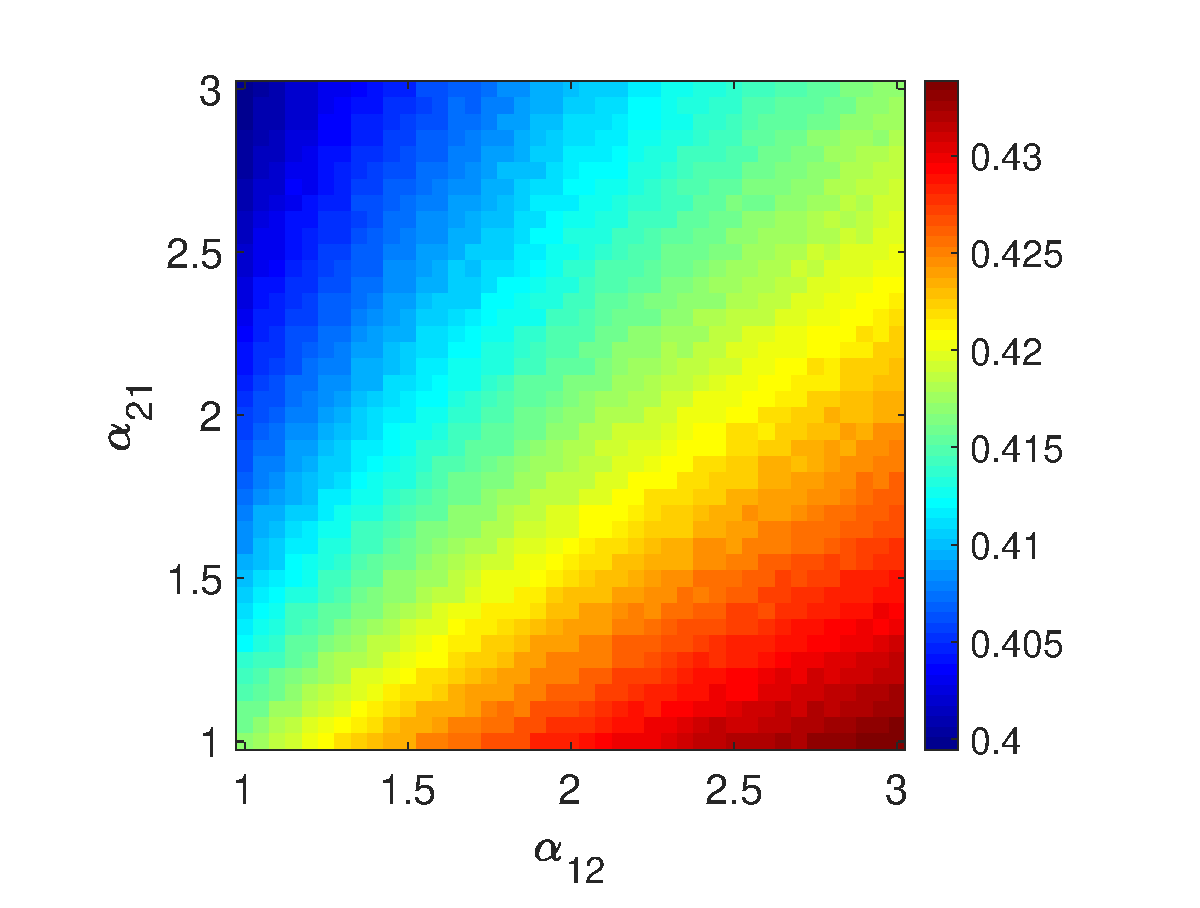
\includegraphics[width=1\linewidth]{Images/photo20_3.eps}
\end{center}

  \end{minipage} 
  
   \caption{\textbf{Amplitude LS on the connectivity parameter space in non-symmetrical homogeneous two-cell networks.} Cell-1 oscillates with amplitude value 1.5, while cell-2 oscillates with amplitude value 1.25. Left and middle: Amplitude LS. For each pair of cross-connectivity parameters, there are the values of self-connectivity parameters, $\alpha_{11}$ (Left) and $\alpha_{22}$ (Middle), such as both the amplitude value of each cell in the network is preserved. Right: Frequency for each point of the amplitude LS. Parameter values: $\lambda = 1$, $b=1$, $a = 1$, $\omega= 1$.}
  \label{photo20}
\end{figure}

The next statement summarizes the main properties of amplitude LSs on the connectivity parameter space in non-symmetrical homogeneous networks.

\begin{Statement}
Non-symmetrical homogeneous networks show 2-dimensional amplitude level sets on the connectivity parameter space. However, the network frequency is not constant throughout amplitude level sets on the connectivity parameter space. Consequently, non-symmetrical homogeneous networks show 1-dimensional total-degenerated level sets on the connectivity parameter space.
\end{Statement}

The fact that the network frequency is not preserve throughout amplitude LSs on the connectivity parameter in non-symmetrical homogeneous networks is the main difference between non-symmetrical and symmetrical homogeneous networks.

\section{Type-\textrm{I} Heterogeneous Two-cell Networks}
We consider type-\textrm{I} heterogeneous networks in which cells belong to the same individual amplitude and frequency LS. Contrary to homogeneous networks, we found that symmetrical and non-symmetrical type-\textrm{I} heterogeneous networks show similar properties. For the sake of simplicity, we illustrate them in a symmetrical type-\textrm{I} heterogeneous network.

\subsection{Connectivity parameter space}

Fig. (\ref{photo21}) shows how breaking the condition for LSs preservation in type-\textrm{I} heterogeneous networks, Eq. (\ref{e29}), affects individual amplitude and frequency LSs. Here, cross-connectivity parameter are fixed and self-connectivity parameters are perturbed from it LSs preserving value. Both self-connectivity parameters are perturbed the same amount so as to see the differences between symmetrical homogeneous and symmetrical type-\textrm{I} heterogeneous networks. Top plots show the effect of mutually higher self-connectivity, whereas bottom plots shows the effect of mutually lower self-connectivity. 

\begin{figure}[h]
\centering
  \begin{minipage}{0.45\linewidth}
  \begin{center}
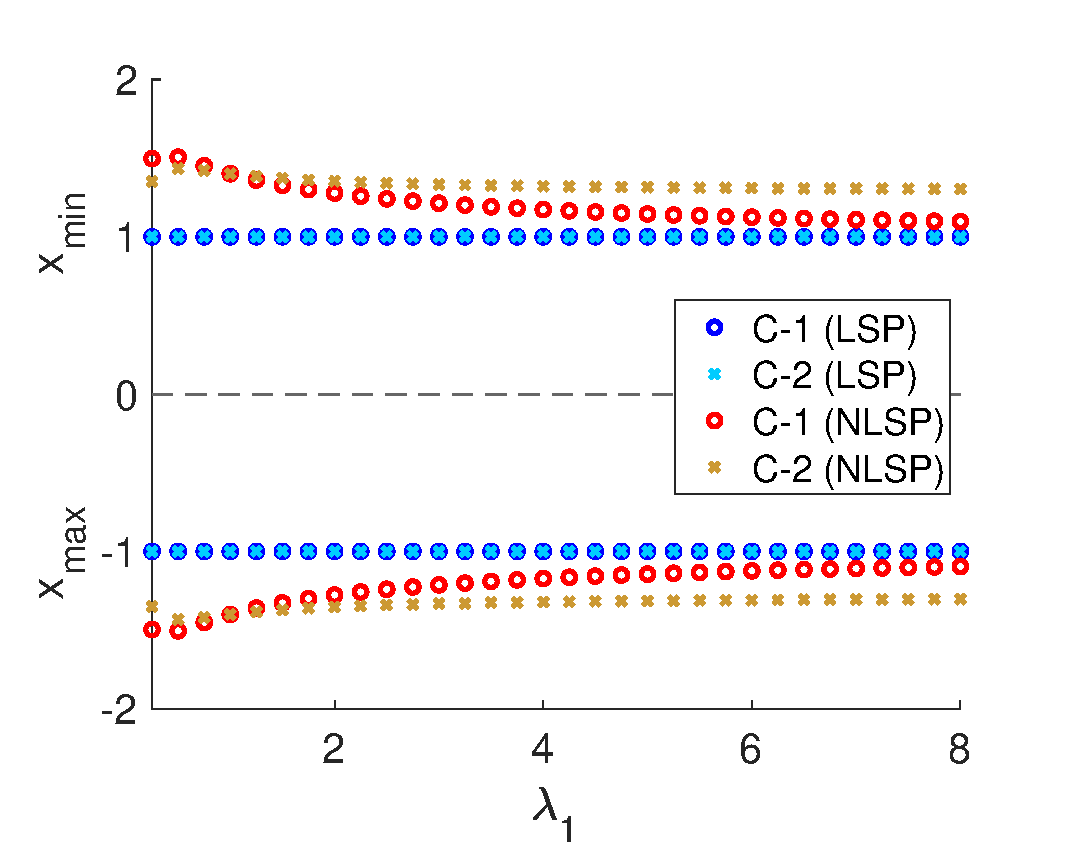
\includegraphics[width=1\linewidth]{Images/photo21_1.eps}
\end{center}
  \end{minipage} 
  \begin{minipage}{0.45\linewidth}
  \begin{center}
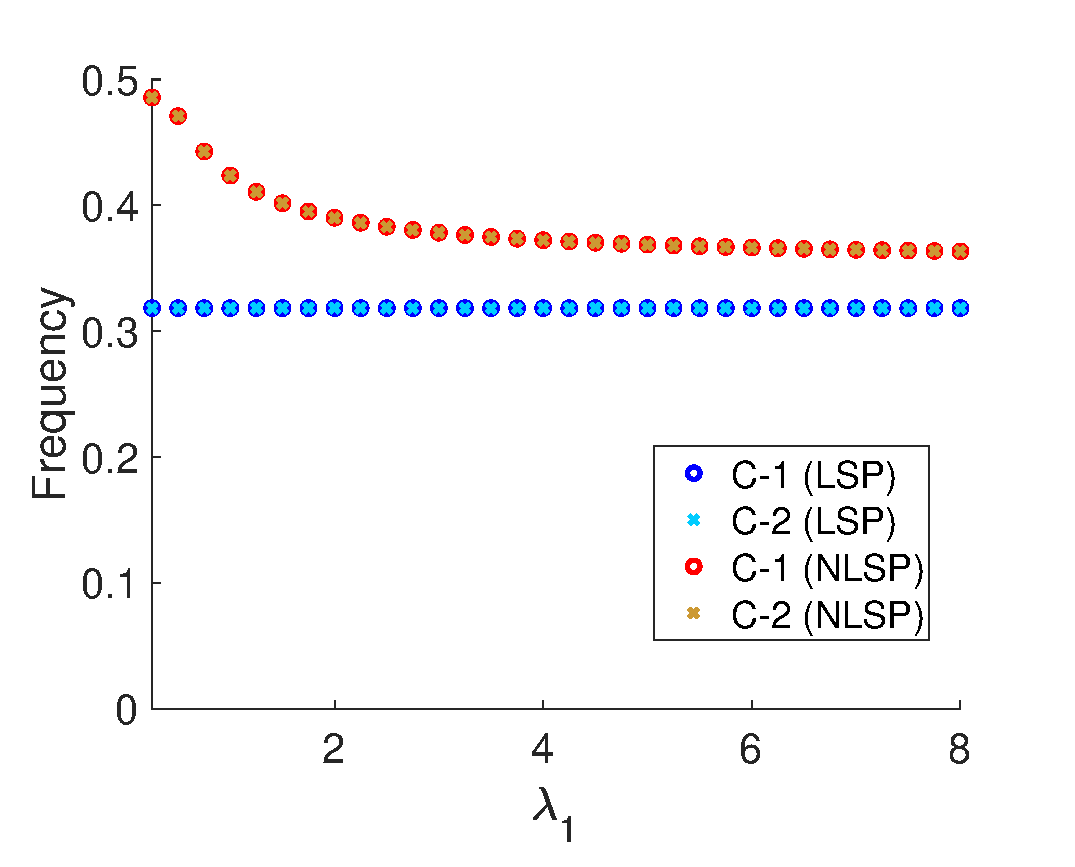
\includegraphics[width=1\linewidth]{Images/photo21_2.eps}
\end{center}
\end{minipage} 
 \begin{minipage}{0.45\linewidth}
  \begin{center}
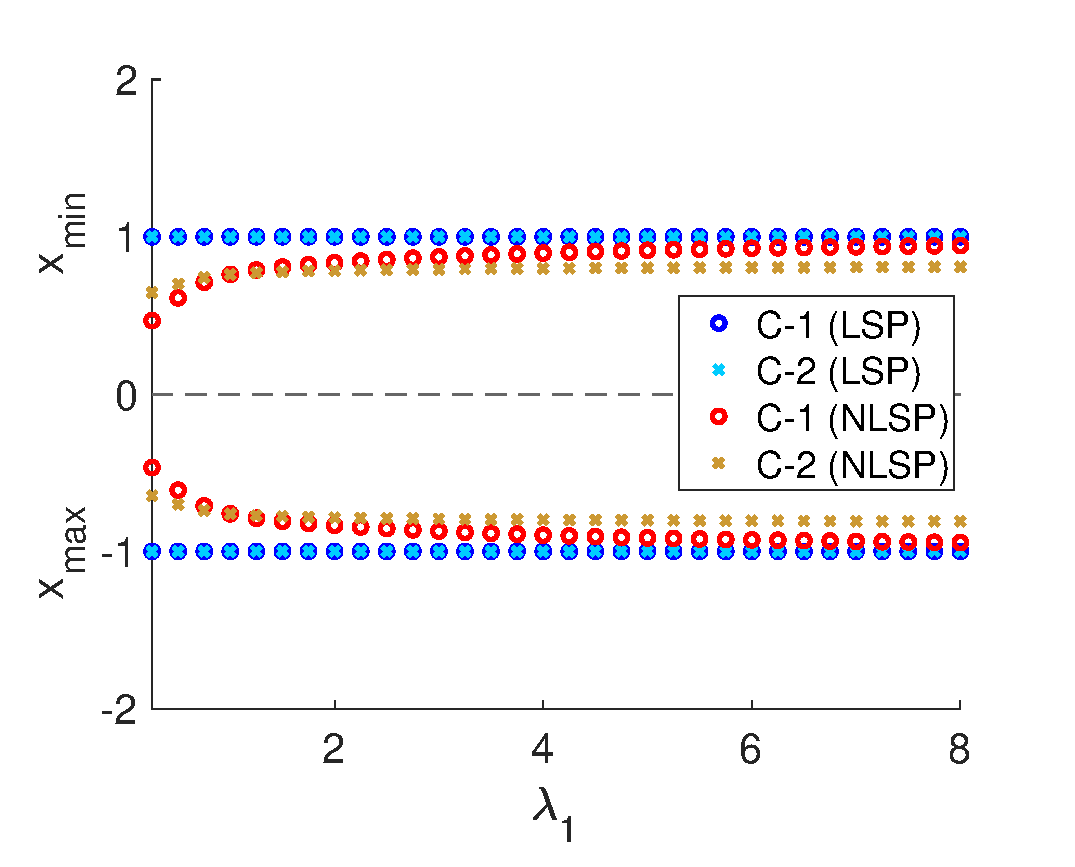
\includegraphics[width=1\linewidth]{Images/photo21_3.eps}
\end{center}
  \end{minipage} 
  \begin{minipage}{0.45\linewidth}
  \begin{center}
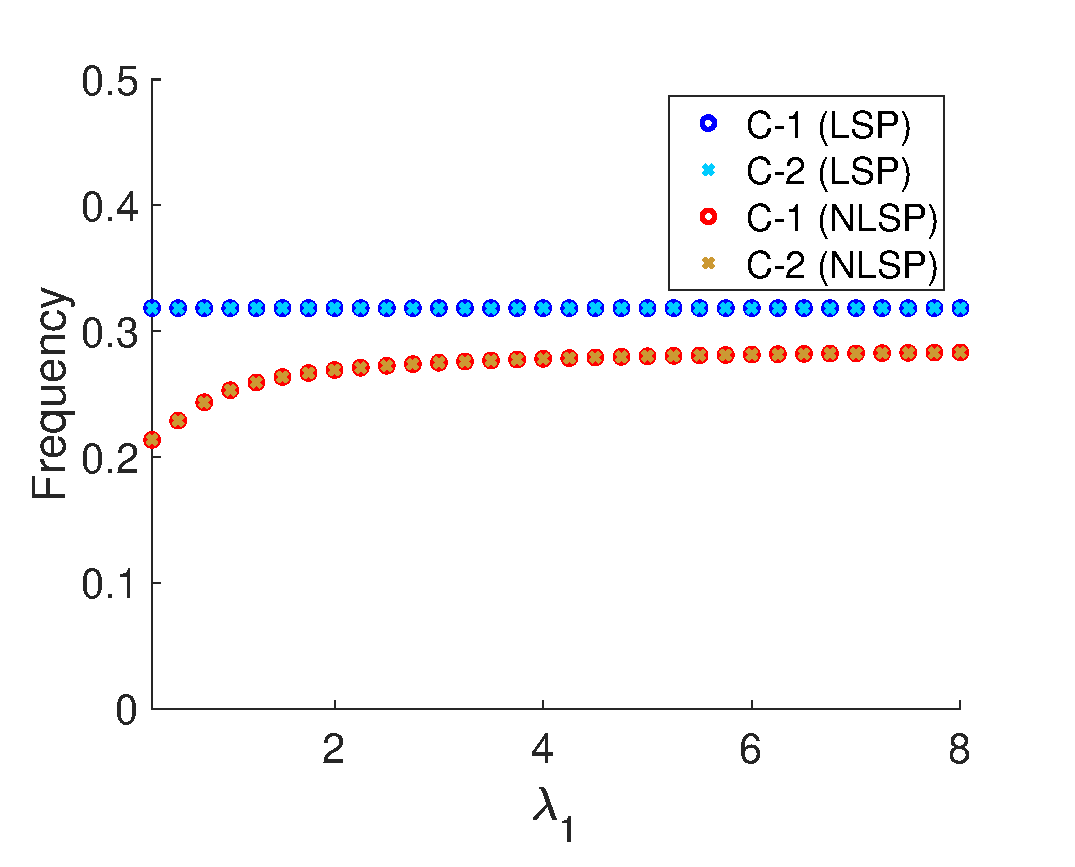
\includegraphics[width=1\linewidth]{Images/photo21_4.eps}
\end{center}
\end{minipage} 
   \caption{\textbf{Effect of mutually higher and lower self-connectivity (compared to the self-connectivity preserving individual LSs) on individual amplitude LSs in synchronized type-\textrm{I} heterogeneous networks.} Top: mutually higher self-connectivity. Parameter values:$\lambda_{2}=1$, $b_{2}=1$, $a = 1$, $\omega = 1$, $\alpha_{12}=1$, $\alpha_{21}=1$, $\alpha_{11}=0.5$ and $\alpha_{22}=0.5$ (Perturbation: $+1.5$). Bottom: mutually lower self-connectivity. Parameter values: $\lambda_{2}=1$, $b_{2}=1$, $a = 1$, $\omega = 1$, $\alpha_{12}=1$, $\alpha_{21}=1$, $\alpha_{11}=-1.75$ and $\alpha_{22}=-1.75$ (Perturbation $-0.75$). Left: amplitude  envelope  diagram  for values  $(\lambda_{1},b_{1})$  belonging  to the  same individual  amplitude LS. Right: frequency  diagram  for  values  $(\lambda_{1},b_{1})$ belonging  to  the  same  individual  amplitude LS. LSP refers to the LS preserving network in which connectivity parameters preserve individual LSs. NLSP refers to perturbed networks in which self-connectivity parameters have been modified.}
  \label{photo21}
\end{figure}

Contrary to homogeneous networks, the amplitude value of each cell in the network is different. In Fig. (\ref{photo21}), the only case in which amplitude values coincide is when cells are identical, which corresponds to the homogeneous network case.

Fig. (\ref{photo22}) shows an example of an amplitude LS ($A_{Net} = 1.5$) on the connectivity parameter space in a type-\textrm{I} heterogeneous network ($K_{a}=1$).

\begin{figure}[h]
  \begin{minipage}{0.32\linewidth}
  \begin{center}
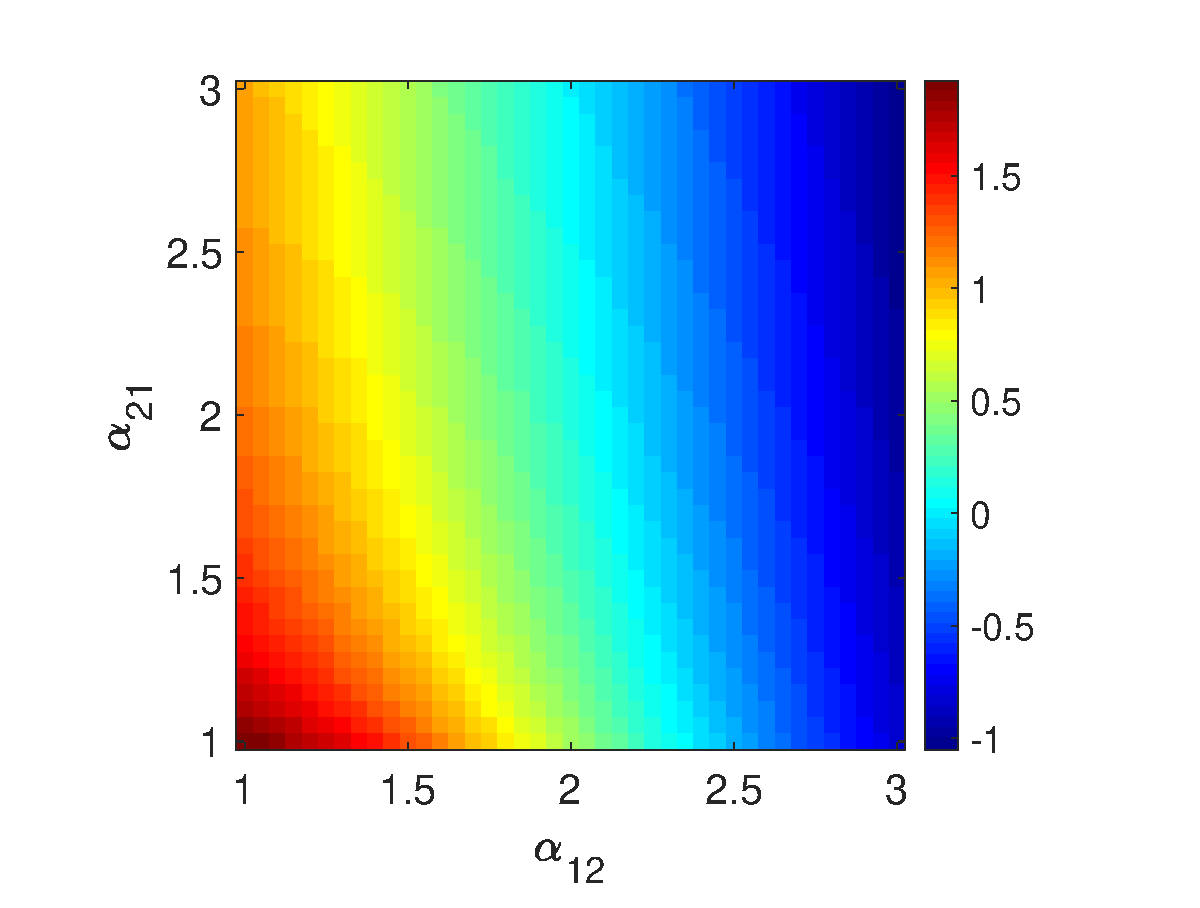
\includegraphics[width=1\linewidth]{Images/photo22_1.eps}
\end{center}
  \end{minipage} 
  \begin{minipage}{0.32\linewidth}
  \begin{center}
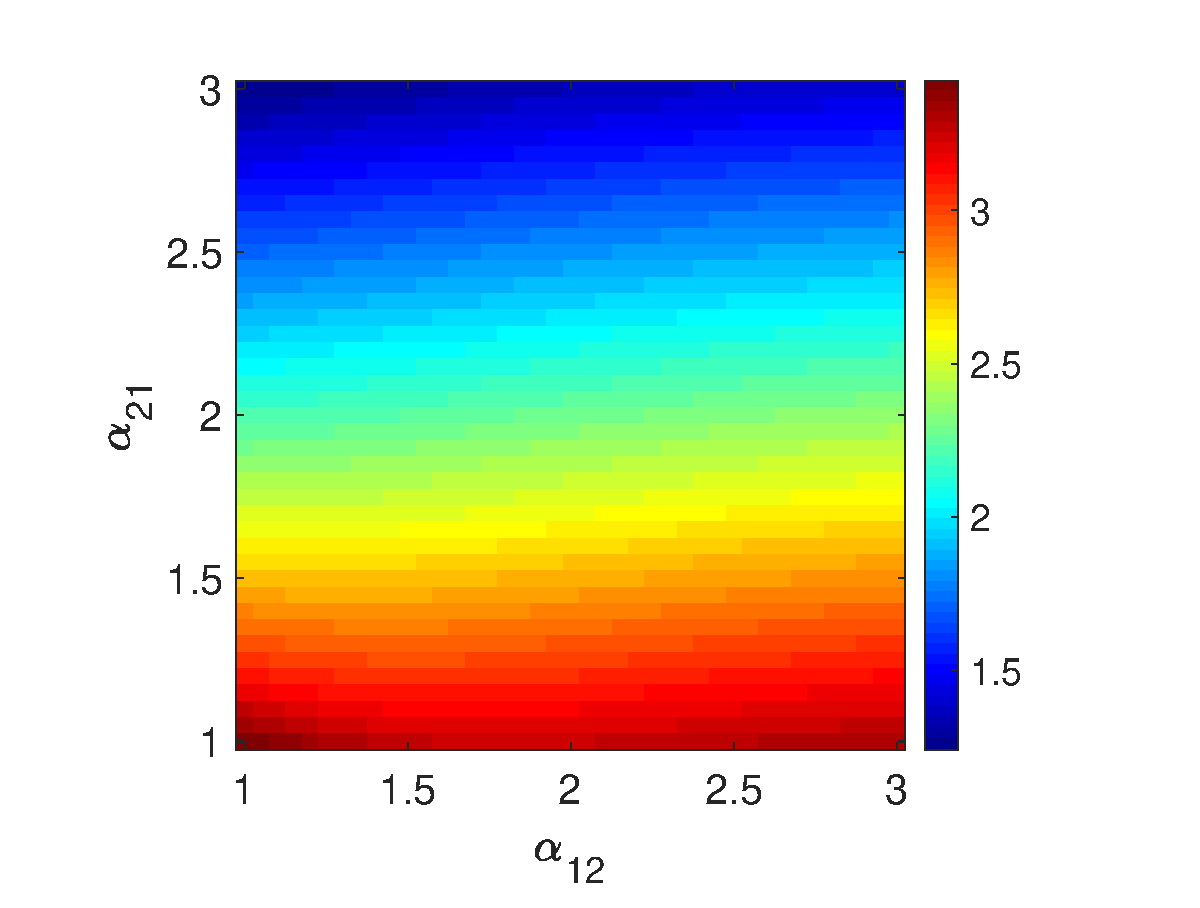
\includegraphics[width=1\linewidth]{Images/photo22_2.eps}
\end{center}

  \end{minipage} 
   \begin{minipage}{0.32\linewidth}
  \begin{center}
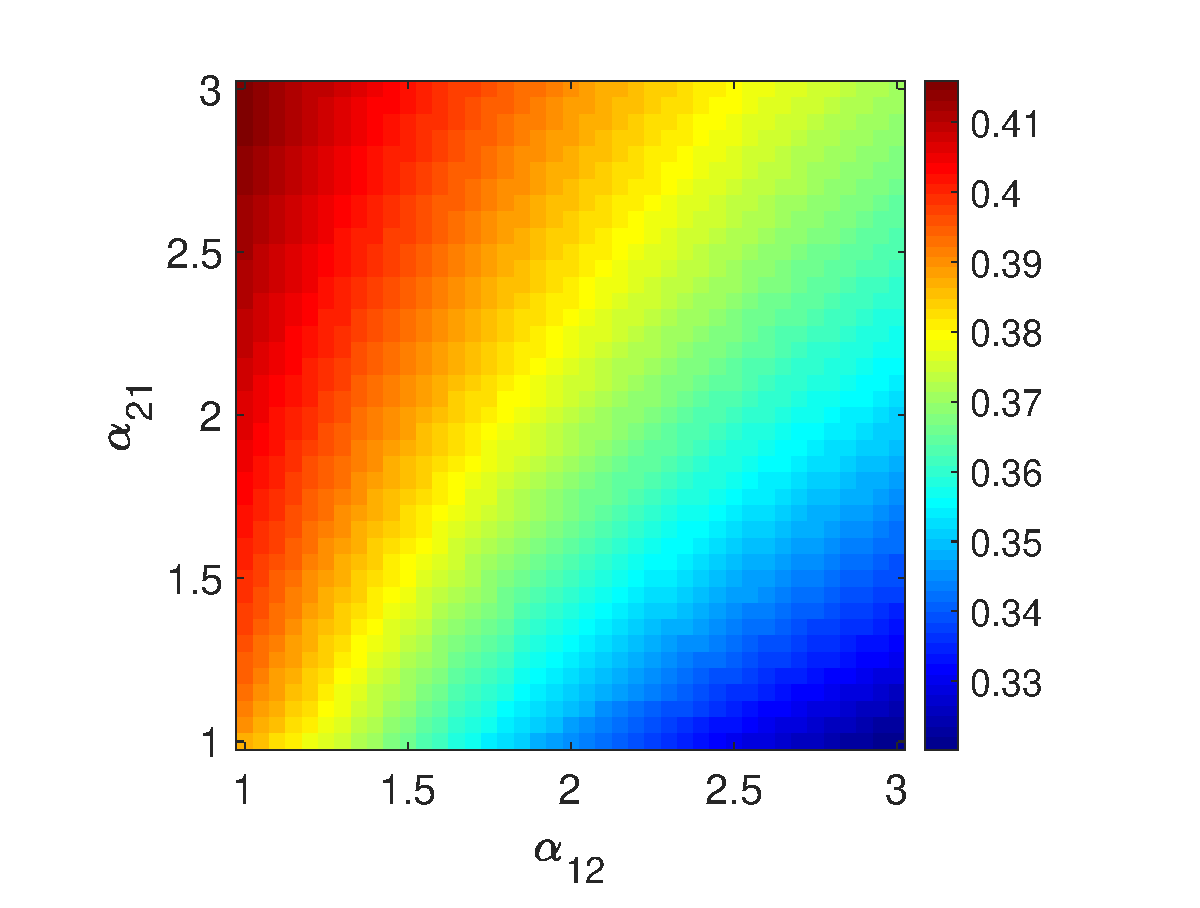
\includegraphics[width=1\linewidth]{Images/photo22_3.eps}
\end{center}

  \end{minipage} 
  
   \caption{\textbf{Amplitude LS on the connectivity parameter space in symmetrical type-\textrm{I} heterogeneous two-cell network.} Both cells oscillate with amplitude value 1.5. Left and middle: amplitude LS. For each pair of cross-connectivity parameters, there are the values of self-connectivity parameters, $\alpha_{11}$ (Left) and $\alpha_{22}$ (Middle), such as the amplitude value of each cell in the network is preserved. Right: frequency for each point on the amplitude LS. Parameter values: $\lambda_{1} = 1$, $b_{1}=1$, $\lambda_{2}=3$, $b_{2}=3$, $a_{1} = 1$, $\omega_{1} = 1$, $a_{2}=1$ and $\omega_{2}=1$.}
  \label{photo22}
\end{figure}

The next statement summarizes the main properties of network LSs on the connectivity parameter space in type-\textrm{I} heterogeneous network. We note that LSs properties in type-\textrm{I} heterogeneous network are the same as LSs properties in non-symmetrical homogeneous networks.

\begin{Statement}
Type-\textrm{I} heterogeneous networks show 2-dimensional amplitude level sets on the connectivity parameter space. However, the network frequency is not constant throughout amplitude level sets on the connectivity parameter space. Consequently, type-\textrm{I} heterogeneous networks show 1-dimensional total-degenerated level sets on the connectivity parameter space.
\end{Statement}

The representative amplitude LS on the connectivity parameter space shown in Fig. (\ref{photo22}) is parametrized by cross-connectivity parameters. We focus on the compensatory relations between compensating parameters $\alpha_{12}$ and $\alpha_{21}$ and compensated parameters $\alpha_{11}$ and $\alpha_{22}$.

Fig. (\ref{photo23}) shows how connectivity parameter are compensated when cross-connectivity parameters are changed in order to preserve the network attributes. Furthermore, voltage traces are shown for two different point on the 1-dimensional total-degenerated LS.

\begin{figure}[h]
  \begin{minipage}{0.32\linewidth}
  \begin{center}
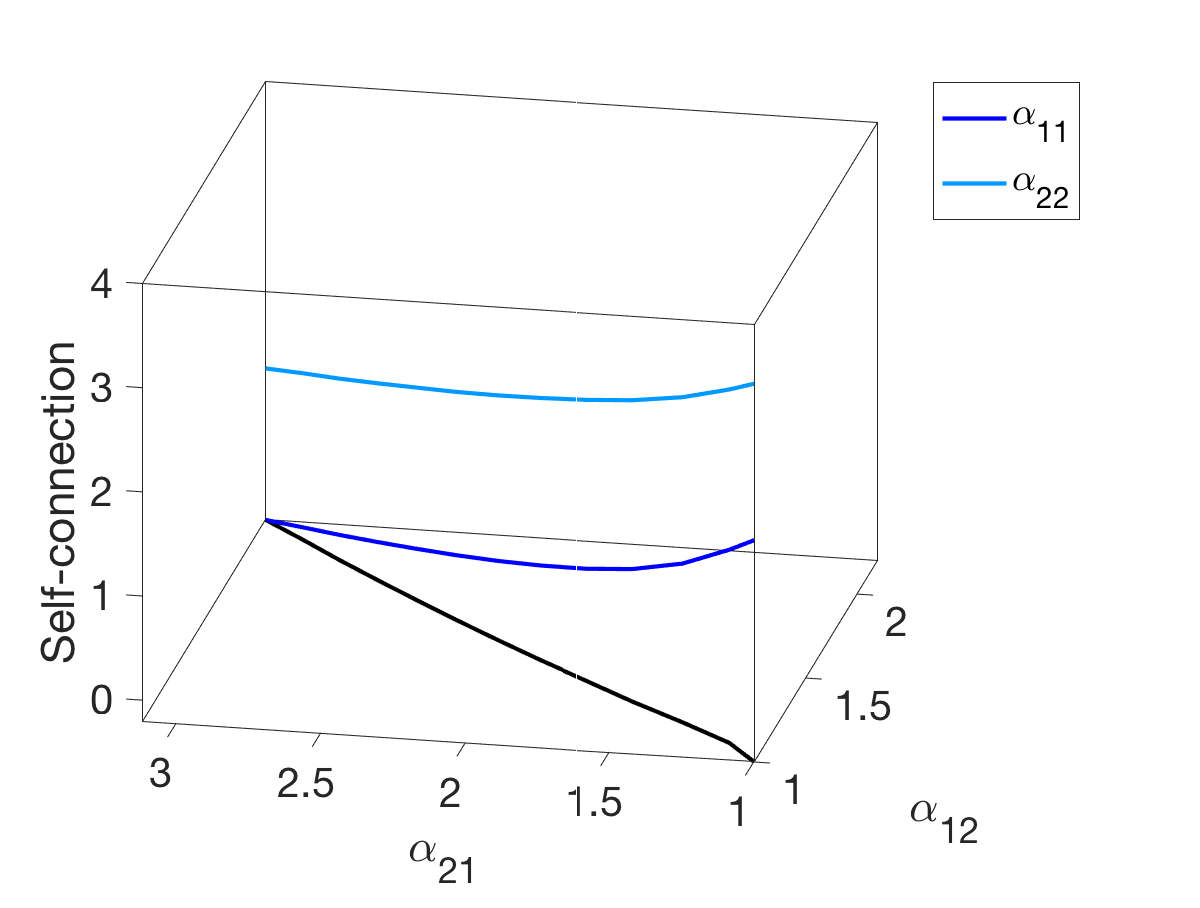
\includegraphics[width=1\linewidth]{Images/photo23_1.eps}
\end{center}
  \end{minipage} 
  \begin{minipage}{0.32\linewidth}
  \begin{center}
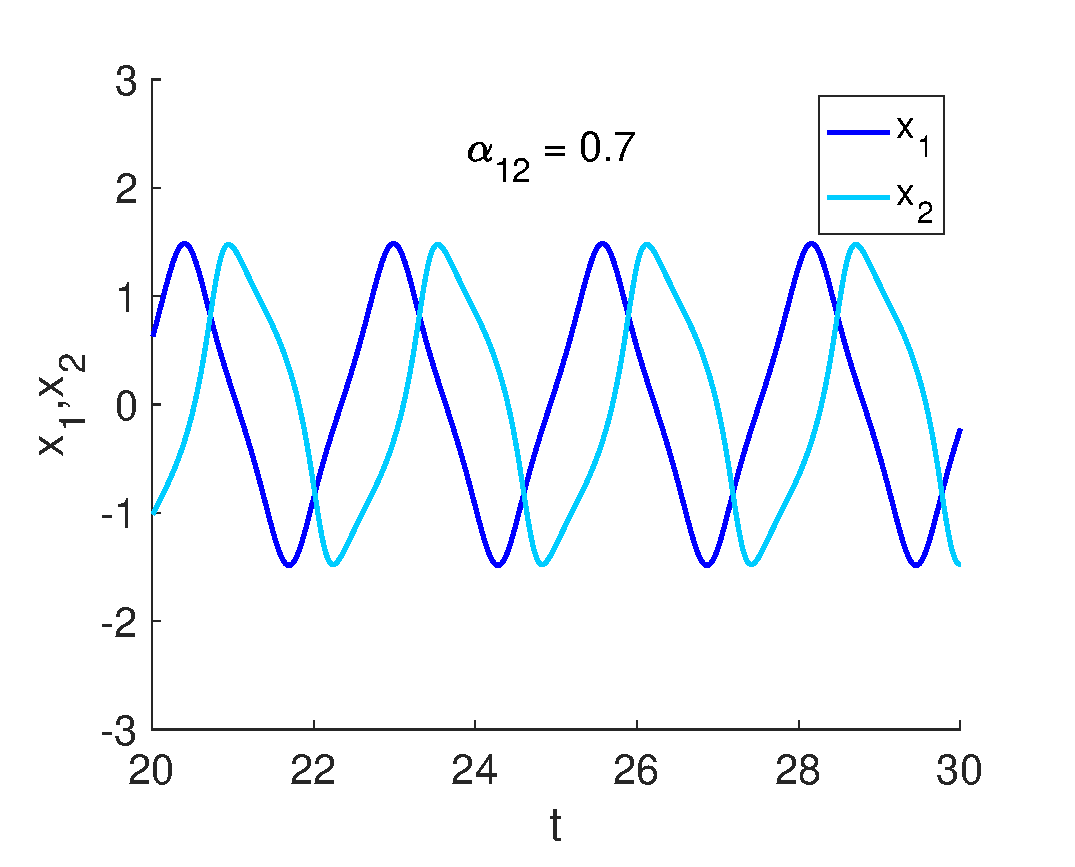
\includegraphics[width=1\linewidth]{Images/photo23_2.eps}
\end{center}

  \end{minipage} 
   \begin{minipage}{0.32\linewidth}
  \begin{center}
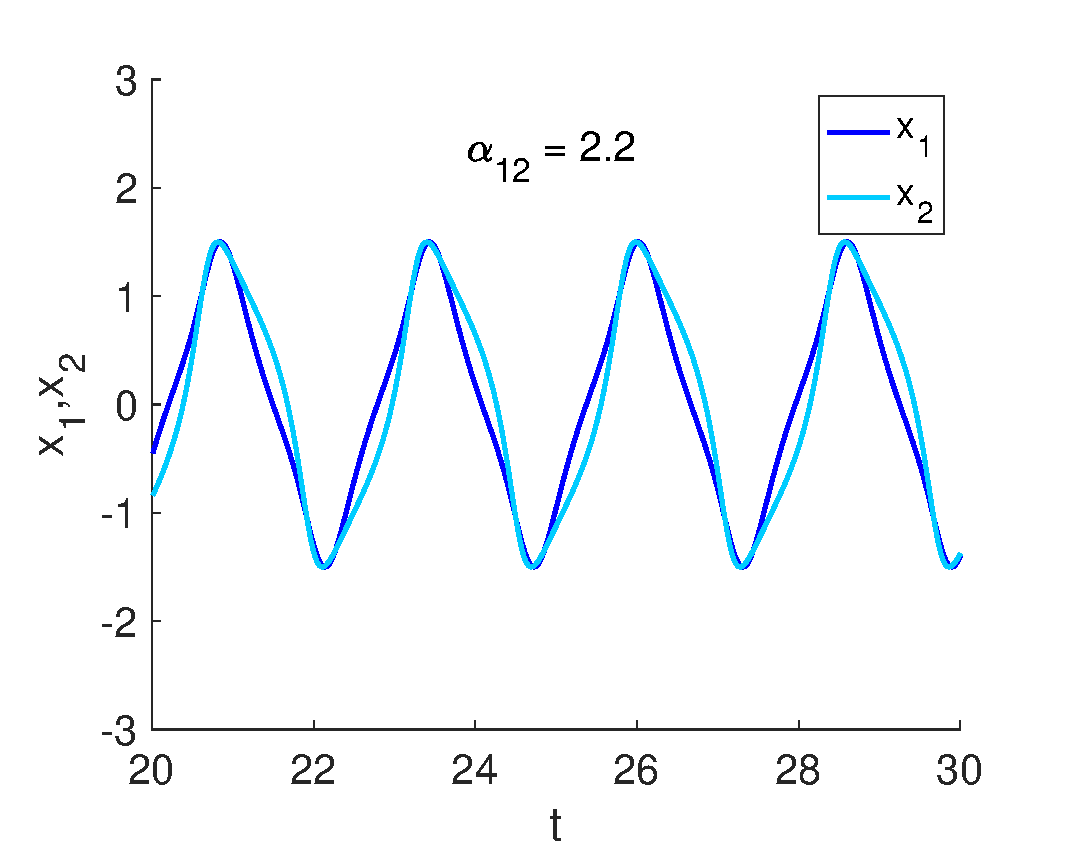
\includegraphics[width=1\linewidth]{Images/photo23_3.eps}
\end{center}

  \end{minipage} 
  
   \caption{\textbf{Total-degenerated LS on the connectivity parameter space.} Network amplitude, $A_{\text{Net}} = 1.5$ and network frequency, $f_{\text{Net}} = 0.37$. Left: total-degenerated LS parametrized by either cross-connectivity parameter. Black line represents the projection of compensated self-connectivity parameters onto the cross-connectivity parameter space. Middle: voltage traces at the point of the LS with $\alpha_{12}=0.7$. Left: voltage traces at the point of the LS with $\alpha_{12}=2.2$. Parameter values: $\lambda_{1} = 1$, $b_{1}=1$, $\lambda_{2}=3$, $b_{2}=3$, $a_{1} = 1$, $\omega_{1} = 1$, $a_{2}=1$ and $\omega_{2}=1$.}
  \label{photo23}
\end{figure}

As it is shown, the increase of any self-connectivity parameter leads to a decrease in its corresponding self-connectivity parameter. For instance, if parameter $\alpha_{12}$ increases, the self-connectivity parameter $\alpha_{11}$ decreases. In addition, the increase of any cross-connectivity parameter leads to an increase in the other cross-connectivity parameter. These compensations are shown in Figure (\ref{photo23})-Left.

Voltage traces seems to preserve their pattern along the total-degenerated LS on the connectivity parameter space shown in Figure (\ref{photo23})-Left, but a significant change in the phase difference is observed.


\subsection{Changing intrinsic parameters}
Finally, we study the dependence between the network frequency on amplitude LSs on connectivity parameter space and intrinsic parameters. Regions on each amplitude LS in which the network frequency is higher and lower than the individual cell frequency are compared. Since the network is type-\textrm{I} heterogeneous, cells do have the same amplitude and frequency value.

Cross-connectivity parameters $\alpha_{12}$ and $\alpha_{21}$ will be the compensating parameters and amplitude LSs on the connectivity parameters space for the same values on the cross-connectivity parameter space (same subspace) are compared.

Fig. (\ref{photo24}) shows the network frequency on several amplitude LSs ($A_{\text{Net}} = 1.5$) for different type-\textrm{I} heterogeneous networks in which cells belong to different points on the individual amplitude LS with $K_{a}=1$. For each amplitude LS, the dark blue region represents point of the amplitude LS in which the network frequency is higher than the individual cell frequency while the light blue region represents point of the amplitude LS in which the network frequency is lower.

\begin{figure}[h]
\centering
  \begin{minipage}{0.32\linewidth}
  \begin{center}
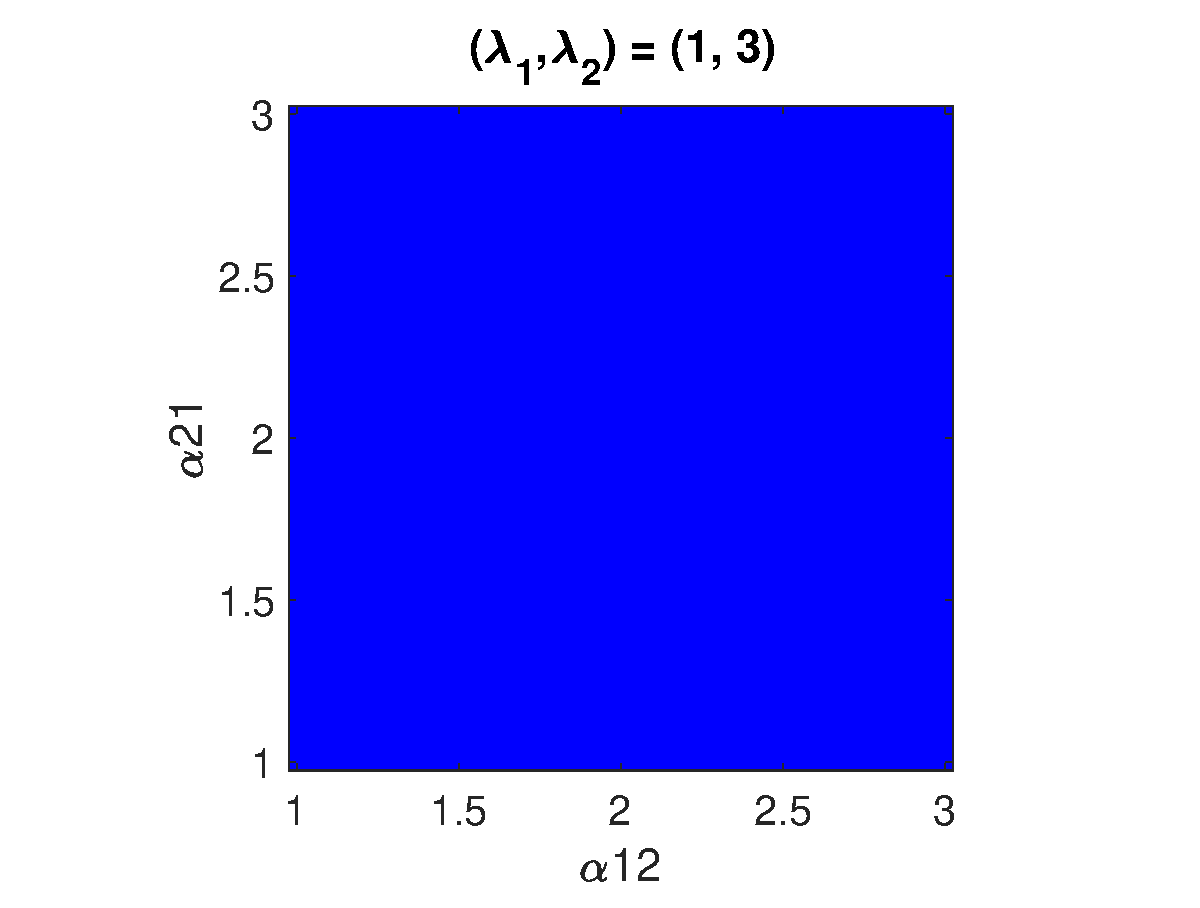
\includegraphics[width=1\linewidth]{Images/photo24_1.eps}
\end{center}
  \end{minipage} 
  \begin{minipage}{0.32\linewidth}
  \begin{center}
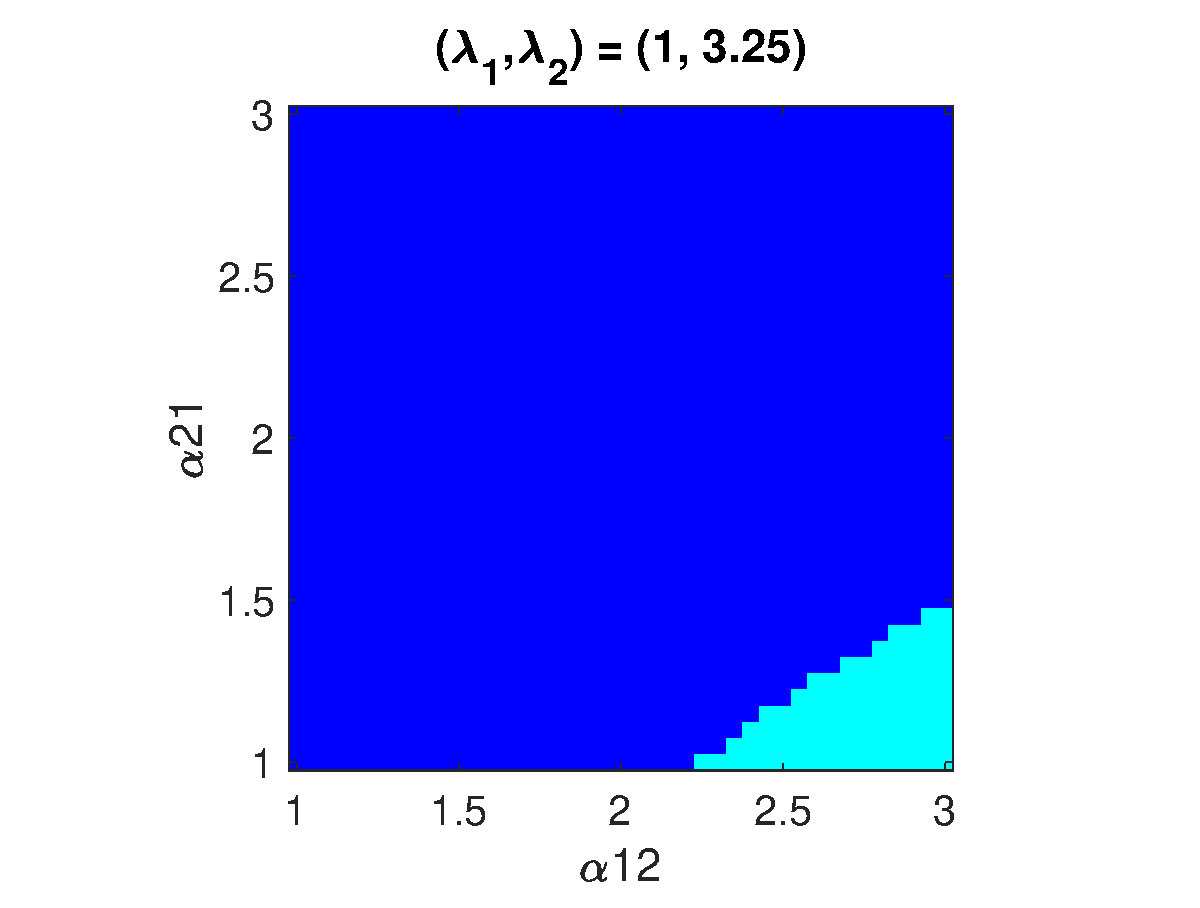
\includegraphics[width=1\linewidth]{Images/photo24_2.eps}
\end{center}

  \end{minipage} 
   \begin{minipage}{0.32\linewidth}
  \begin{center}
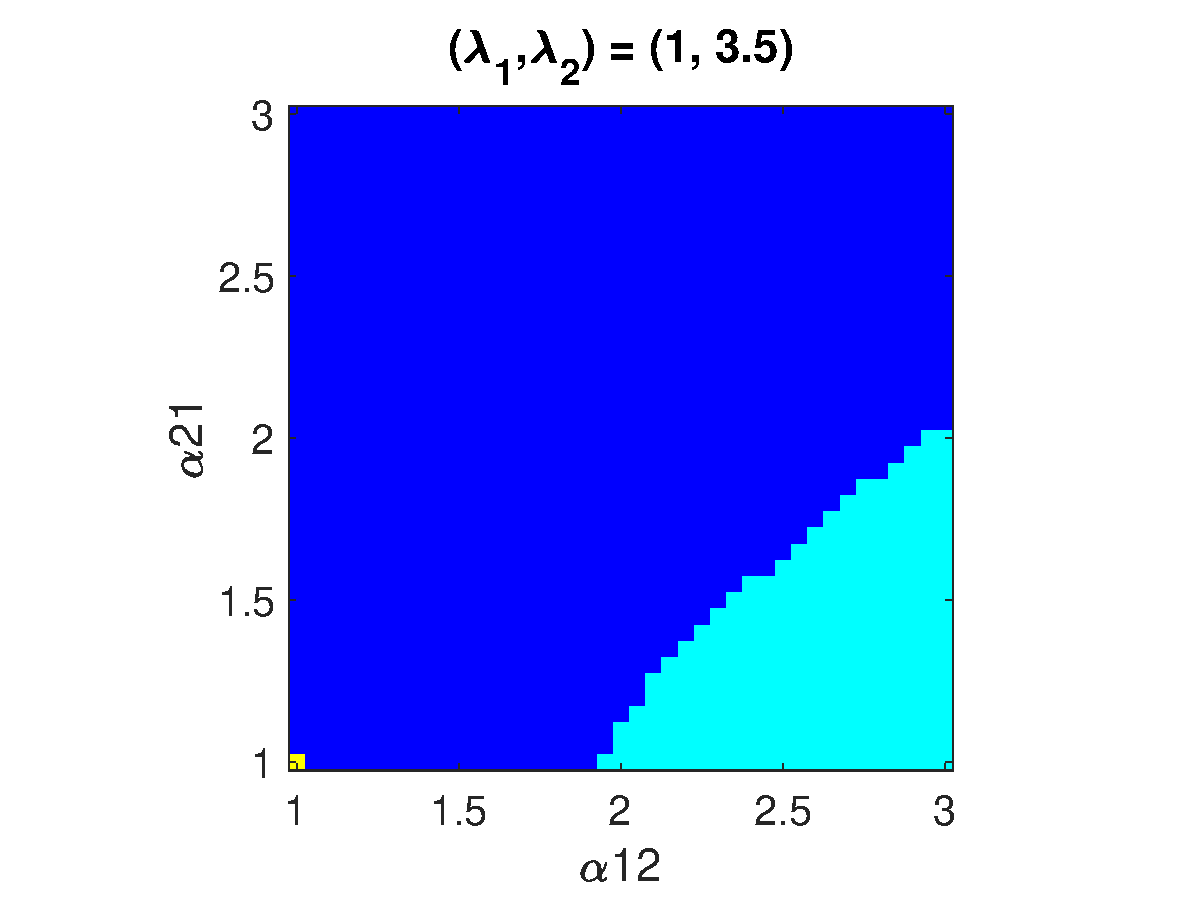
\includegraphics[width=1\linewidth]{Images/photo24_3.eps}
\end{center}
  \end{minipage} 
  
   \begin{minipage}{0.32\linewidth}
  \begin{center}
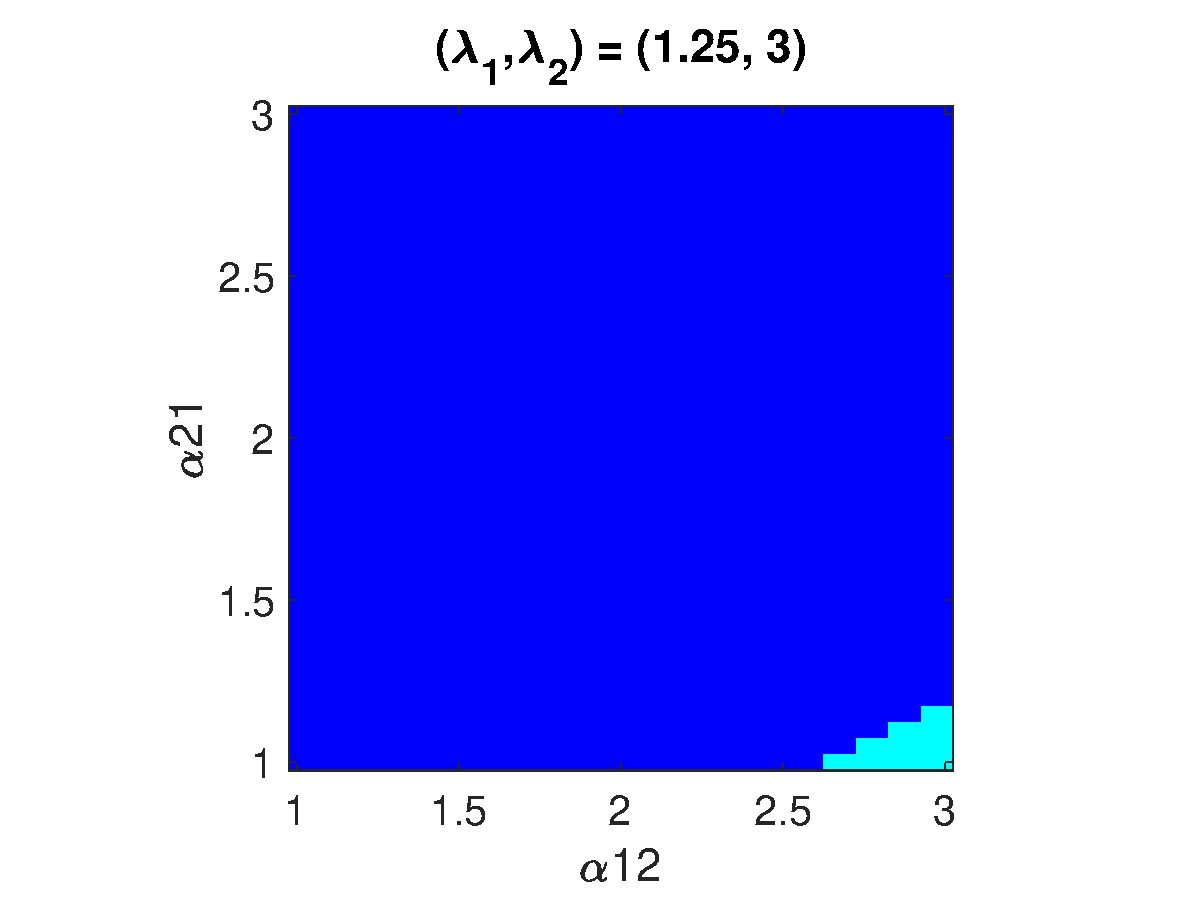
\includegraphics[width=1\linewidth]{Images/photo24_4.eps}
\end{center}
  \end{minipage} 
  \begin{minipage}{0.32\linewidth}
  \begin{center}
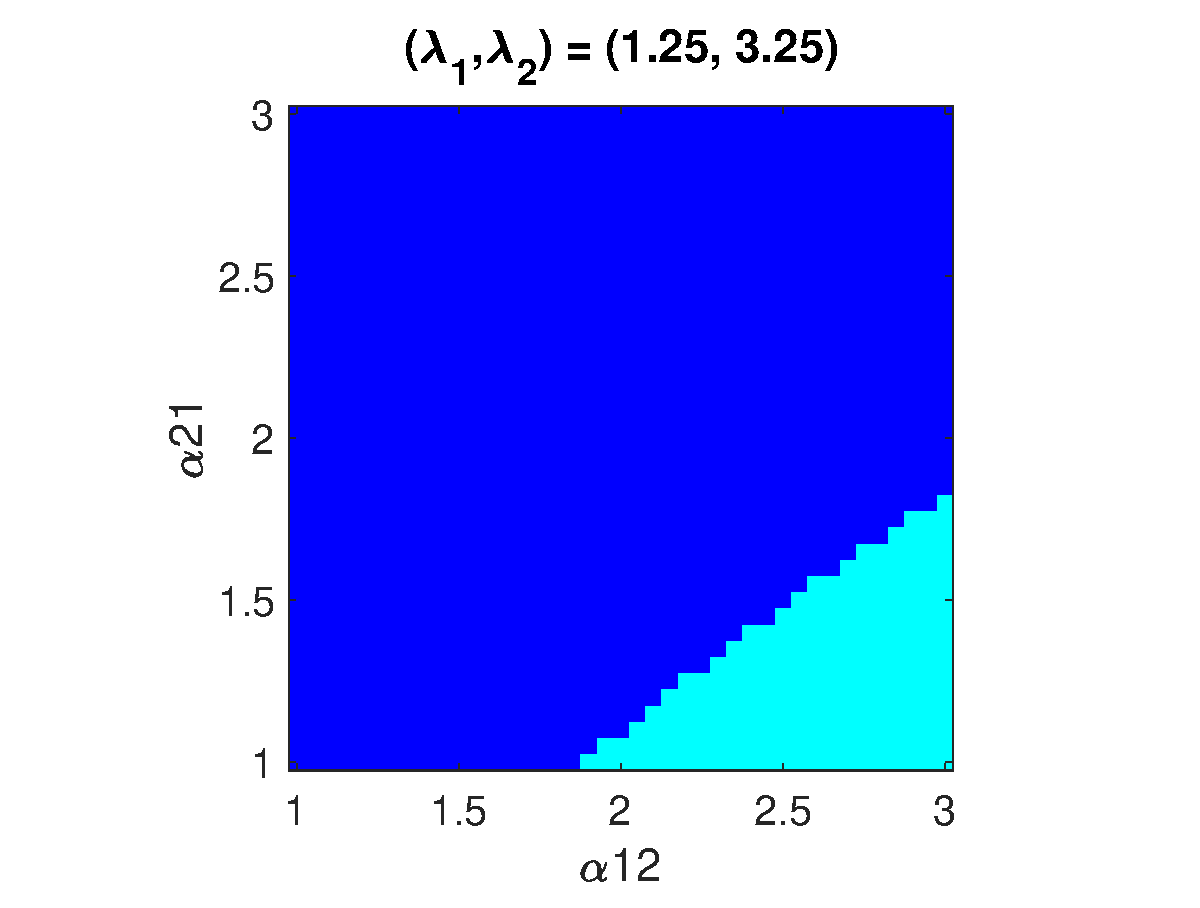
\includegraphics[width=1\linewidth]{Images/photo24_5.eps}
\end{center}

  \end{minipage} 
   \begin{minipage}{0.32\linewidth}
  \begin{center}
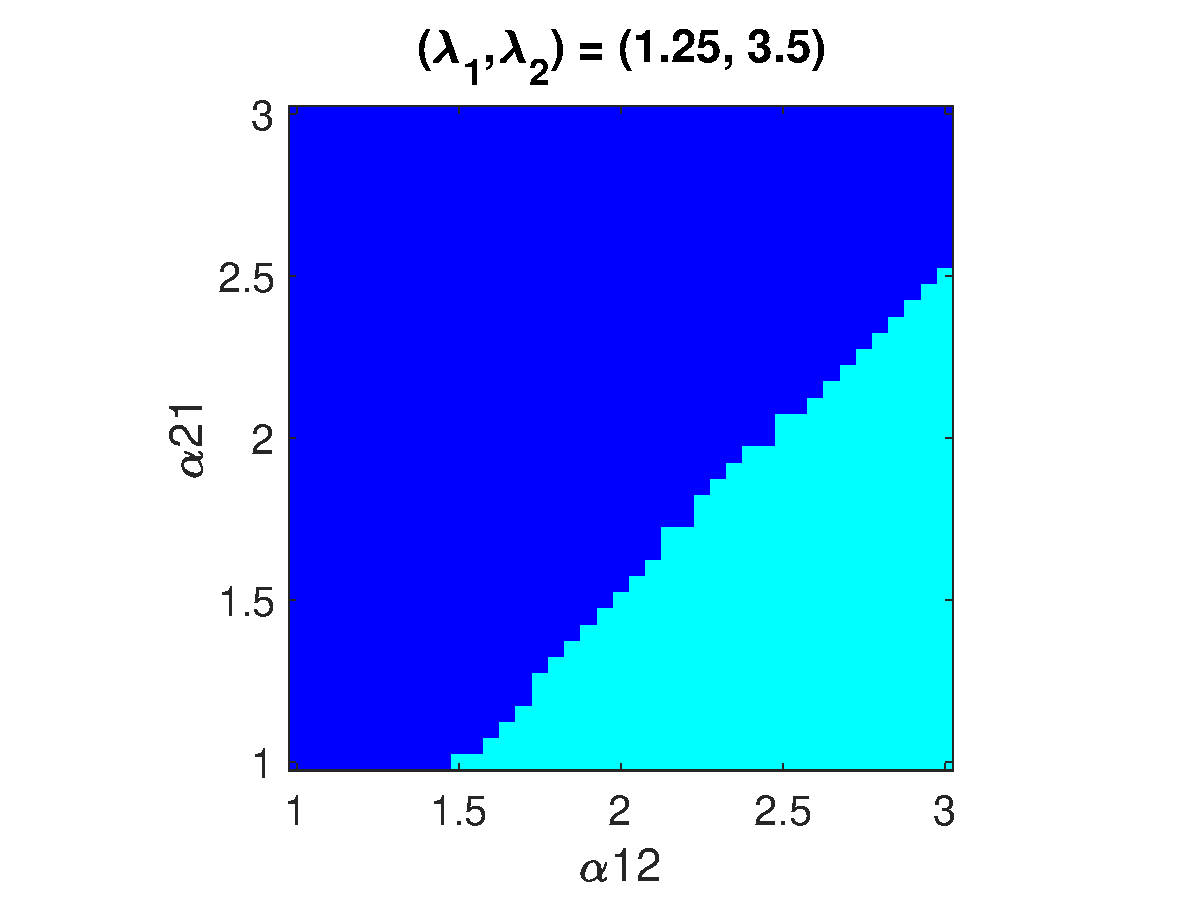
\includegraphics[width=1\linewidth]{Images/photo24_6.eps}
\end{center}
  \end{minipage} 
  
   \begin{minipage}{0.32\linewidth}
  \begin{center}
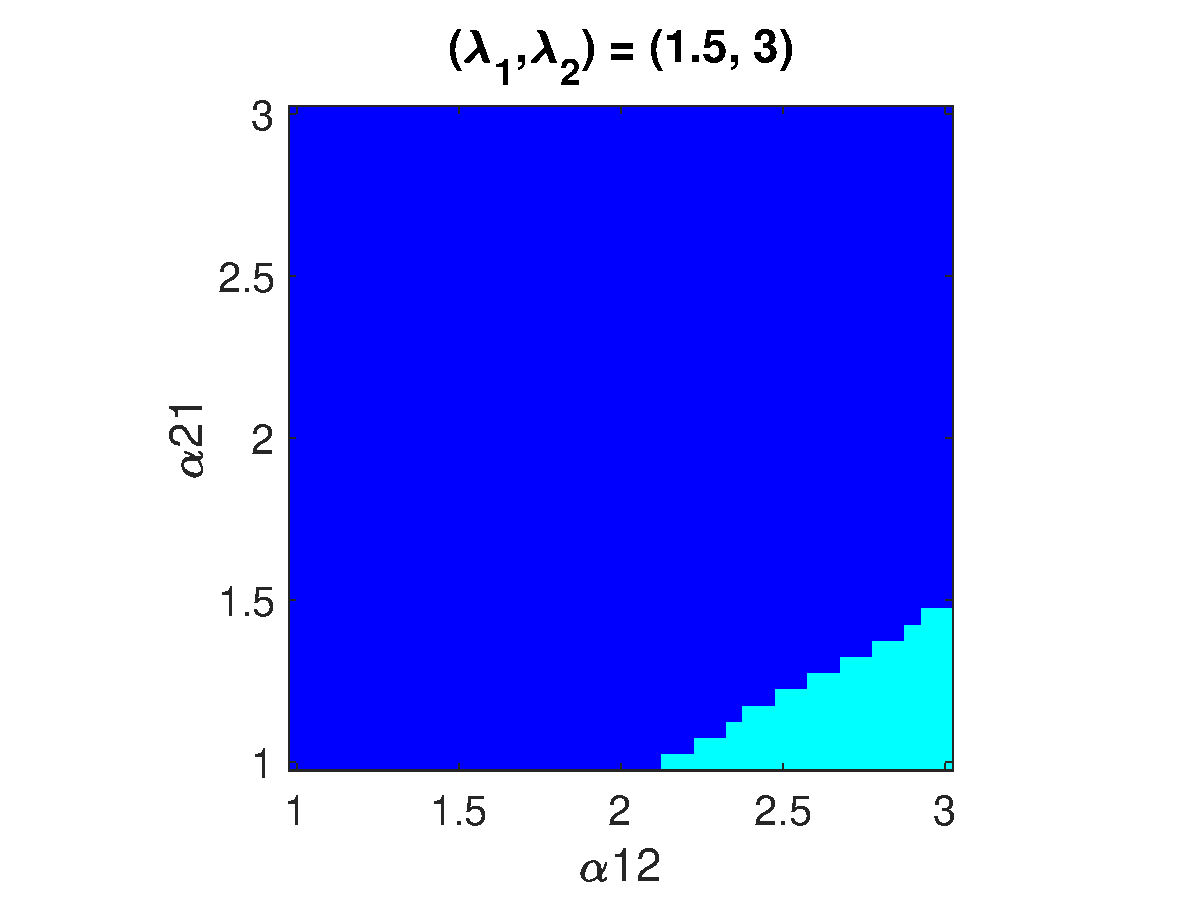
\includegraphics[width=1\linewidth]{Images/photo24_7.eps}
\end{center}
  \end{minipage} 
  \begin{minipage}{0.32\linewidth}
  \begin{center}
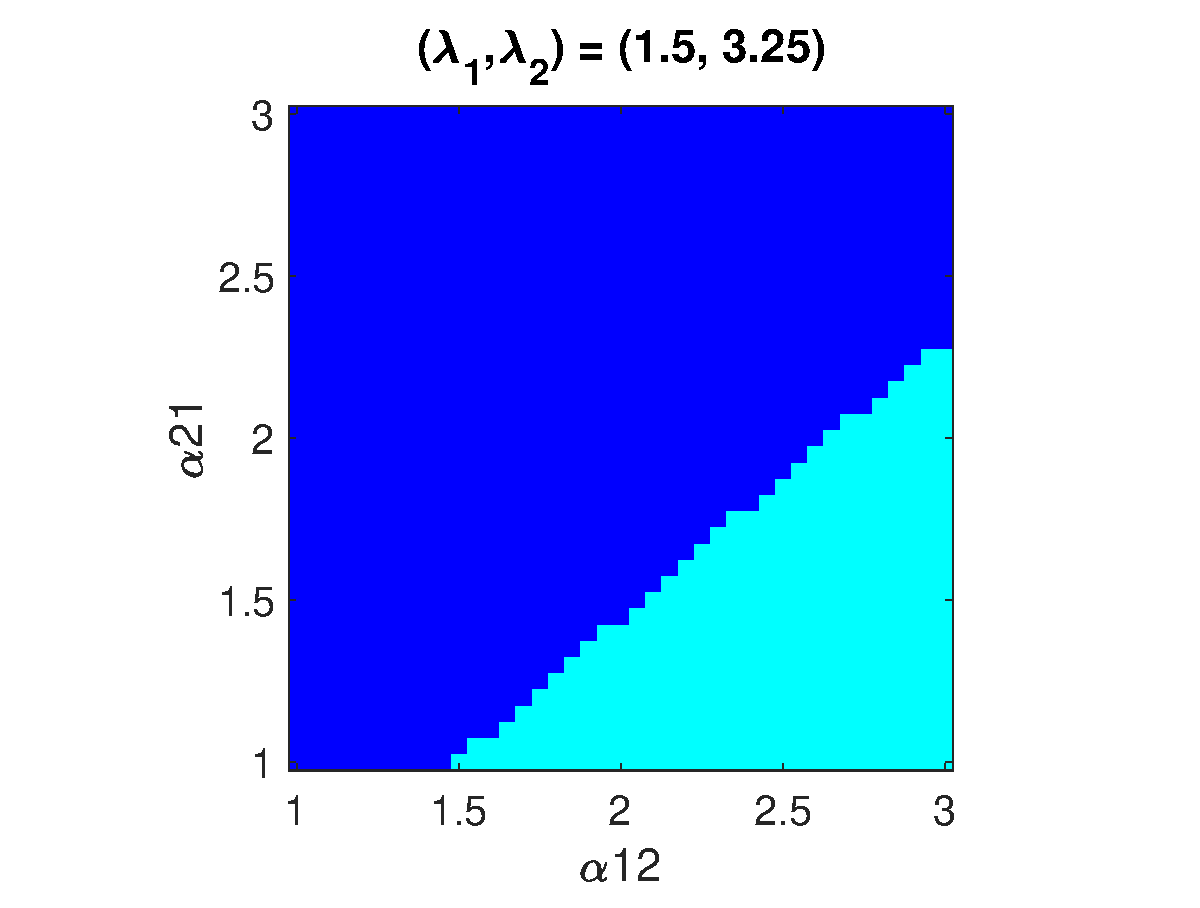
\includegraphics[width=1\linewidth]{Images/photo24_8.eps}
\end{center}

  \end{minipage} 
   \begin{minipage}{0.32\linewidth}
  \begin{center}
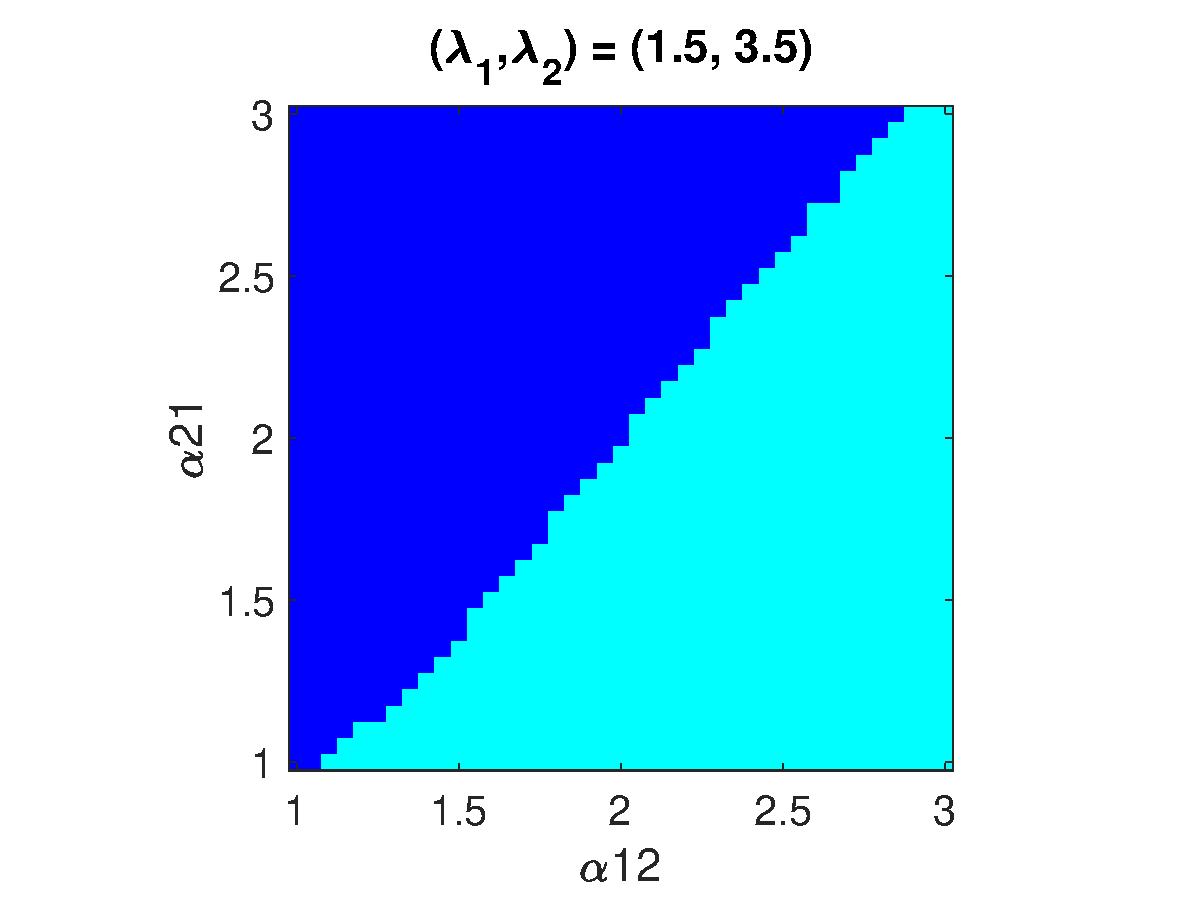
\includegraphics[width=1\linewidth]{Images/photo24_9.eps}
\end{center}
  \end{minipage} 
  
   \caption{\textbf{Intrinsic parameter in type-\textrm{I} heterogeneous two-cell network have an overall effect on the network frequency on amplitude LSs on the connectivity parameter space.} Both cells oscillate with amplitude value 1.5. Both cells belong to different points of the individual amplitude LS with $K_{a}=1$. Rows: cell-2 moves along its individual amplitude LS. Columns: cell-1 moves along its individual amplitude LS. Dark blue represent points in the amplitude LS for which the network amplitude is higher than the individual cell frequency while light blue represents points in the amplitude LS for which the network amplitude is lower than the individual cell frequency. Parameter values: $a_{1} = 1$, $\omega= 1$, $a_{2}=1$ and $\omega_{2}=1$.}
  \label{photo24}
\end{figure}

As a result, as intrinsic parameters $\lambda_{1}$ or $\lambda_{2}$ are higher (cell-1 or cell-2 moves along its individual amplitude LS towards higher values of $\lambda_{1}$ or $\lambda_{2}$), the network frequency on amplitude LSs on the connectivity parameter space decreases and take lower values.

We note that although connectivity parameter are able to change the network frequency on a given amplitude LS, a greater effect on the network frequency is observed when intrinsic parameters $\lambda_{1}$ or $\lambda_{2}$ are changed. Moreover, total degenerated LSs could be found on the $\lambda_{1}-\lambda_{2}-\alpha_{11}-\alpha_{22}$ parameter space as well.


\section{Type-\textrm{II} Heterogeneous Two-cell Networks}
Type-\textrm{II} heterogeneous networks represent the most general network, in which cells belong to different individual amplitude and frequency LSs. Therefore, cells do have different individual amplitude and frequencies values. We will not distinguish between symmetrical and non-symmetrical type-\textrm{II} heterogeneous networks since they show the same network attribute LSs properties.

Firstly, we start characterizing LSs on the connectivity parameter space. Afterwards, we study LSs on the intrinsic parameter space of a single cell. We will study whether or not network attributes can be maintained if only intrinsic parameters of a cell in the network are changed. Finally we show total-degenerated network LSs on a mixed parameter space involving intrinsic parameters from both cells.

\subsection{Connectivity parameter space}
Fig. (\ref{photo25}) shows an example of an amplitude LS ($A_{\text{Net}}$ = 1.5) in an type-\textrm{II} heterogeneous network for representative parameter values. It is also shown the network frequency for each point on the amplitude LS.

\begin{figure}[h]
  \begin{minipage}{0.32\linewidth}
  \begin{center}
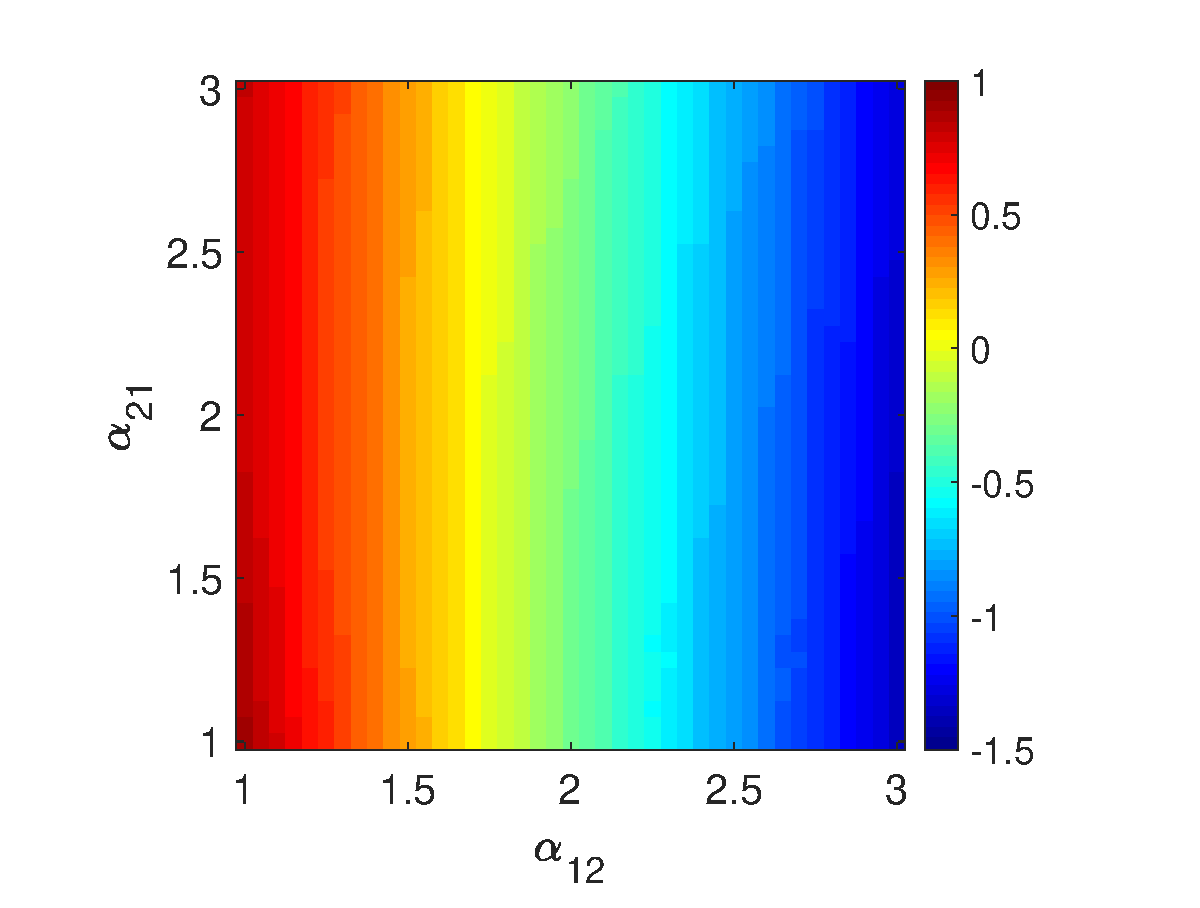
\includegraphics[width=1\linewidth]{Images/photo25_2.eps}
\end{center}
  \end{minipage} 
  \begin{minipage}{0.32\linewidth}
  \begin{center}
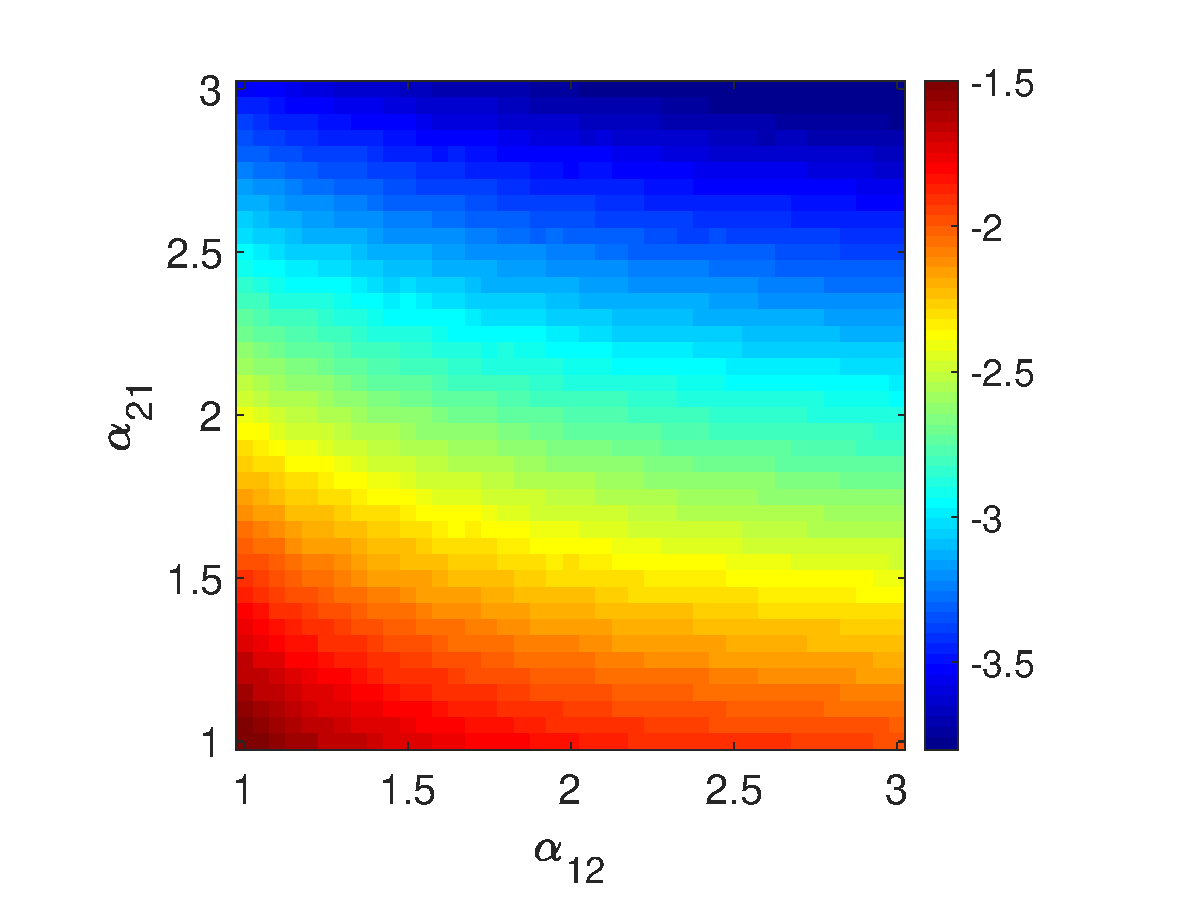
\includegraphics[width=1\linewidth]{Images/photo25_1.eps}
\end{center}

  \end{minipage} 
   \begin{minipage}{0.32\linewidth}
  \begin{center}
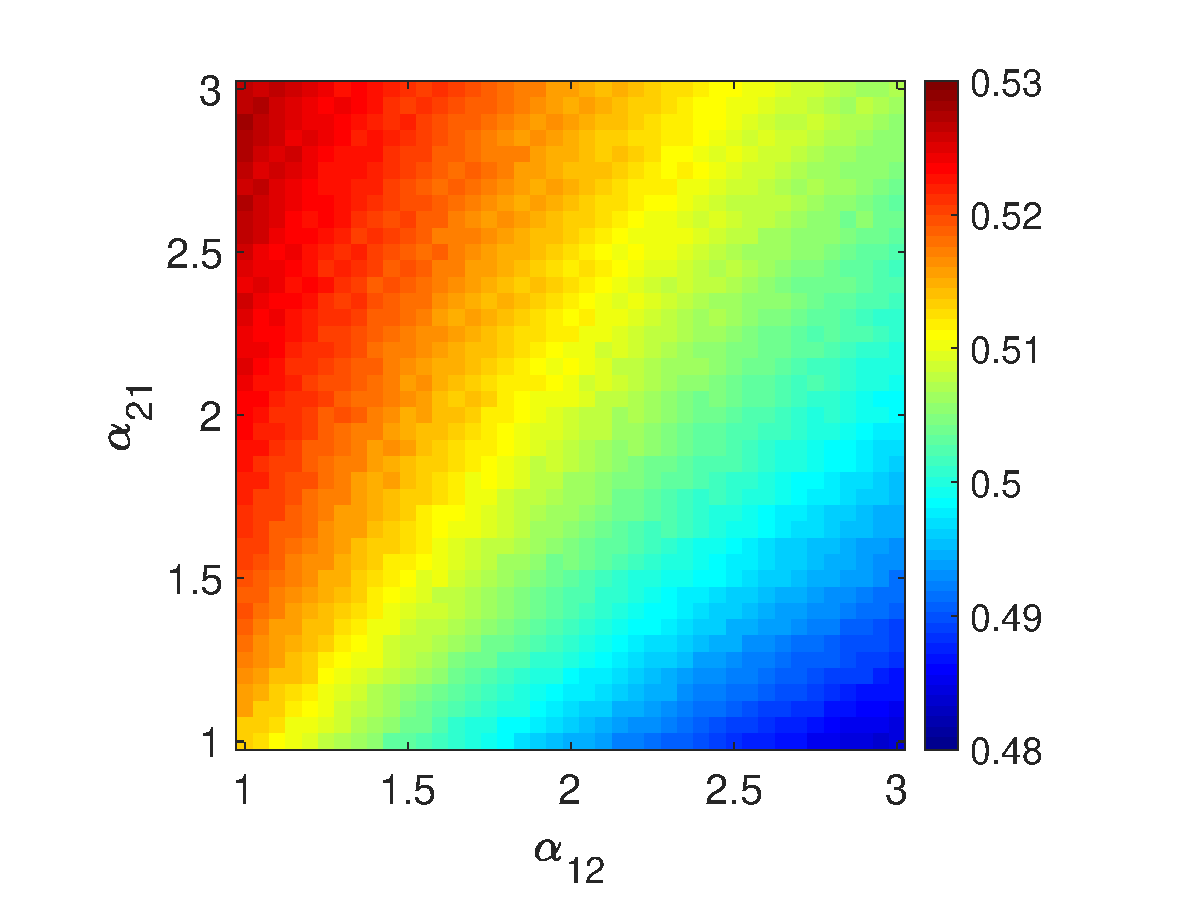
\includegraphics[width=1\linewidth]{Images/photo25_3.eps}
\end{center}

  \end{minipage} 
  
  \caption{\textbf{Amplitude LS on the connectivity parameter space in type-\textrm{II} heterogeneous two-cell network.} Both cells oscillate with amplitude value 1.5. Left and Middle: amplitude LS. For each pair of cross-connectivity parameters, there are the values of self-connectivity parameters, $\alpha_{11}$ (Left) and $\alpha_{22}$ (Middle), such as both the amplitude value of each cell in the network is preserved. Right: frequency for each point of the amplitude LS. Parameter values: $\lambda_{1} = 1$, $b_{1}=1$, $a_{1} = 1$, $\omega_{1} = 1$, $\lambda_{2} = 3$, $b_{2}=1$, $a_{2} = 1$, $\omega_{2} = 1$.}
  \label{photo25}
\end{figure}

The next Statement summarizes the main LSs properties on the connectivity parameter space in type-\textrm{II} heterogeneous networks.

\begin{Statement}
Type-\textrm{II} heterogeneous networks show 2-dimensional amplitude level sets on the connectivity parameter space. However, the network frequency is not constant throughout amplitude level sets on the connectivity parameter space. Consequently, type-\textrm{II} heterogeneous networks show 1-dimensional total-degenerated level sets on the connectivity parameter space.
\end{Statement}

We note type-\textrm{I} and type-\textrm{II} heterogeneous networks show similar network LSs properties on the connectivity parameter space. Both show 1-dimensional total-generated LSs on the connectivity parameter space.

\subsection{The intrinsic parameter space of a single cell}
An interesting question in type-\textrm{II} heterogeneous networks is whether intrinsic parameters of a cell can be changed preserving network attributes. In other words, is it possible to find total-degenerated LSs on the intrinsic parameter space of a single cell?. Without loss of generality we consider the $\lambda_{1}-b_{1}-\omega_{1}-a_{1}$ parameter space, which corresponds to the intrinsic parameter space of cell-1.

Fig. (\ref{photo26}) shows an example of a LS on the  $\lambda_{1}-b_{1}-\omega_{1}-a_{1}$ parameter space preserving the network frequency ($f_{\text{Net}}$) and amplitude of cell-1 ($A_{1}$). It is also shown the amplitude value of cell-2 ($A_{2}$) for each point on the LS. In particular, curves on the LS preserving the amplitude value of cell-2 represent total-degenerated LSs on the intrinsic parameter space of cell-1.

\begin{figure}[h]
  \begin{minipage}{0.32\linewidth}
  \begin{center}
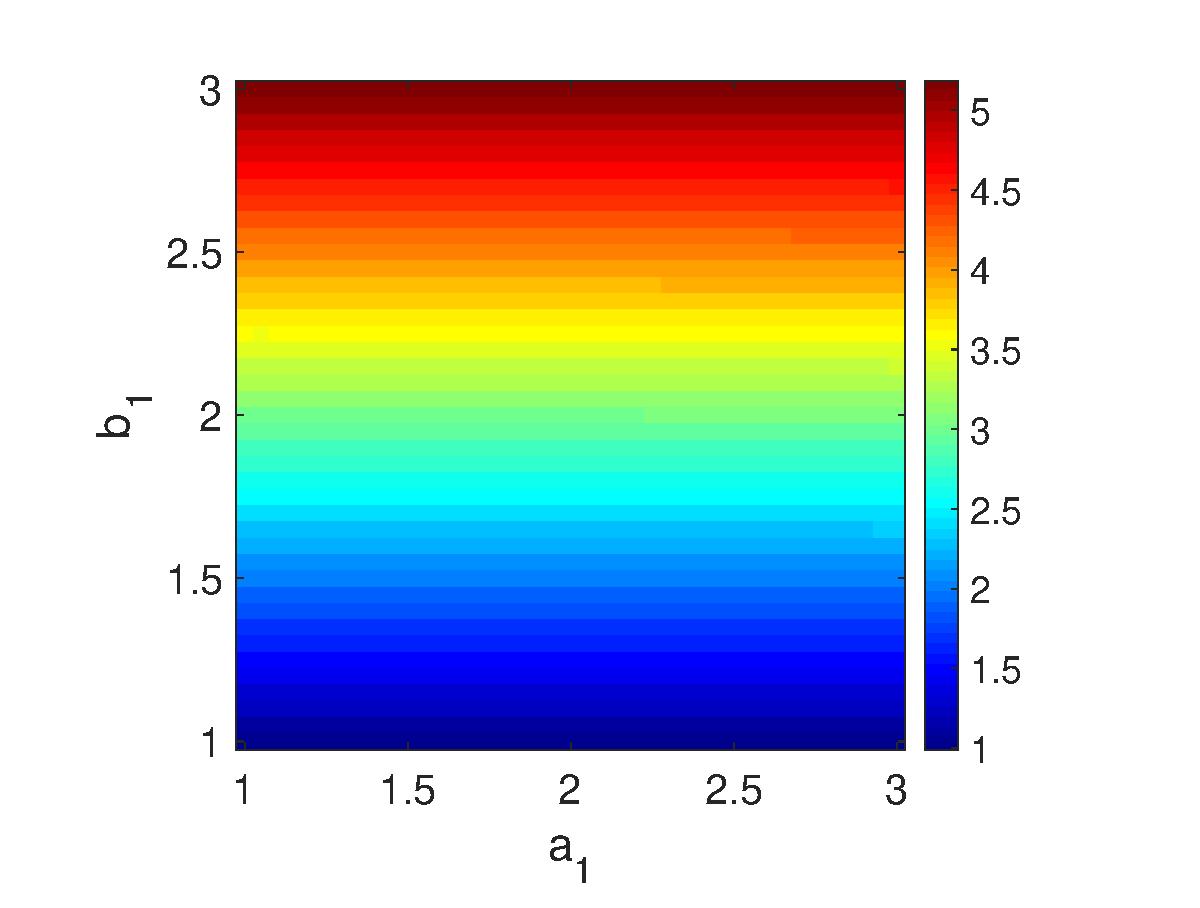
\includegraphics[width=1\linewidth]{Images/photo26_1.eps}
\end{center}
  \end{minipage} 
  \begin{minipage}{0.32\linewidth}
  \begin{center}
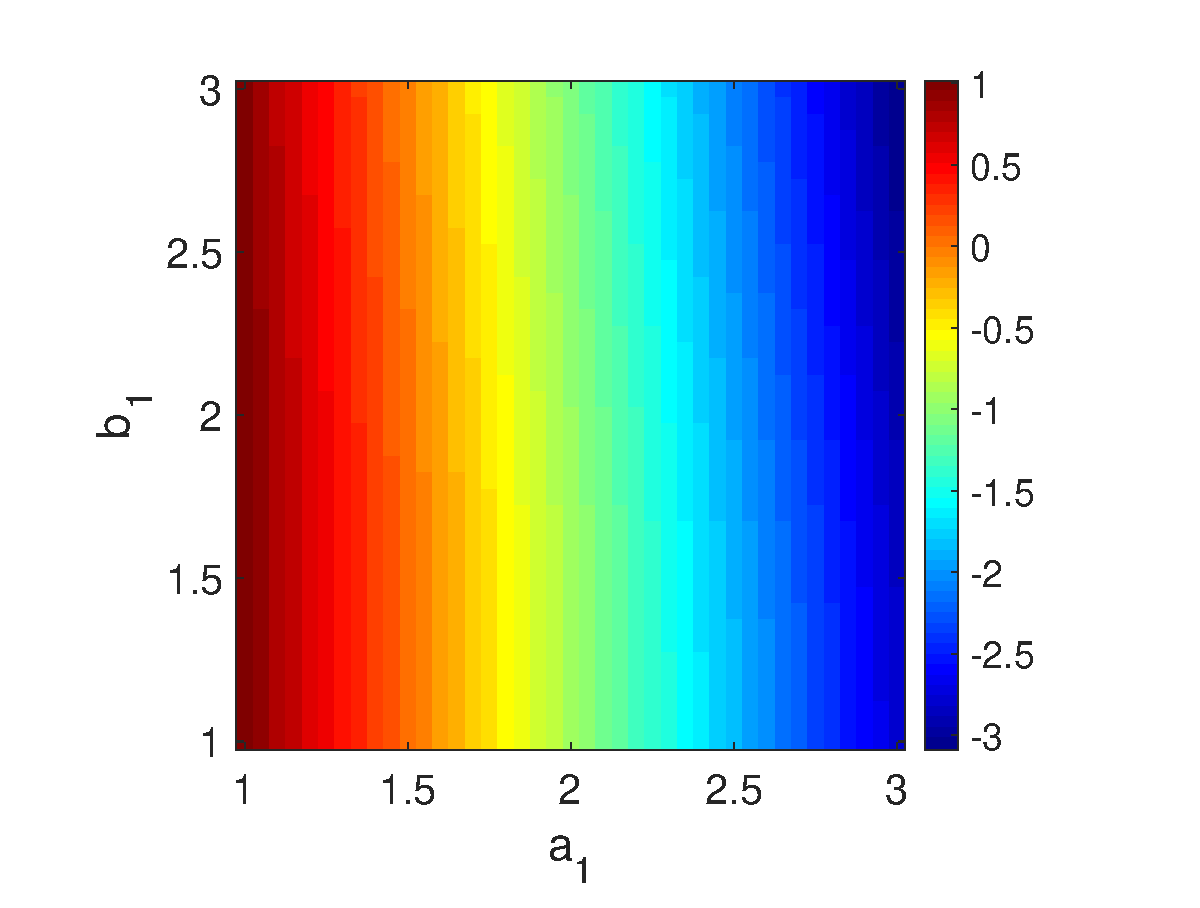
\includegraphics[width=1\linewidth]{Images/photo26_2.eps}
\end{center}
  \end{minipage} 
   \begin{minipage}{0.32\linewidth}
  \begin{center}
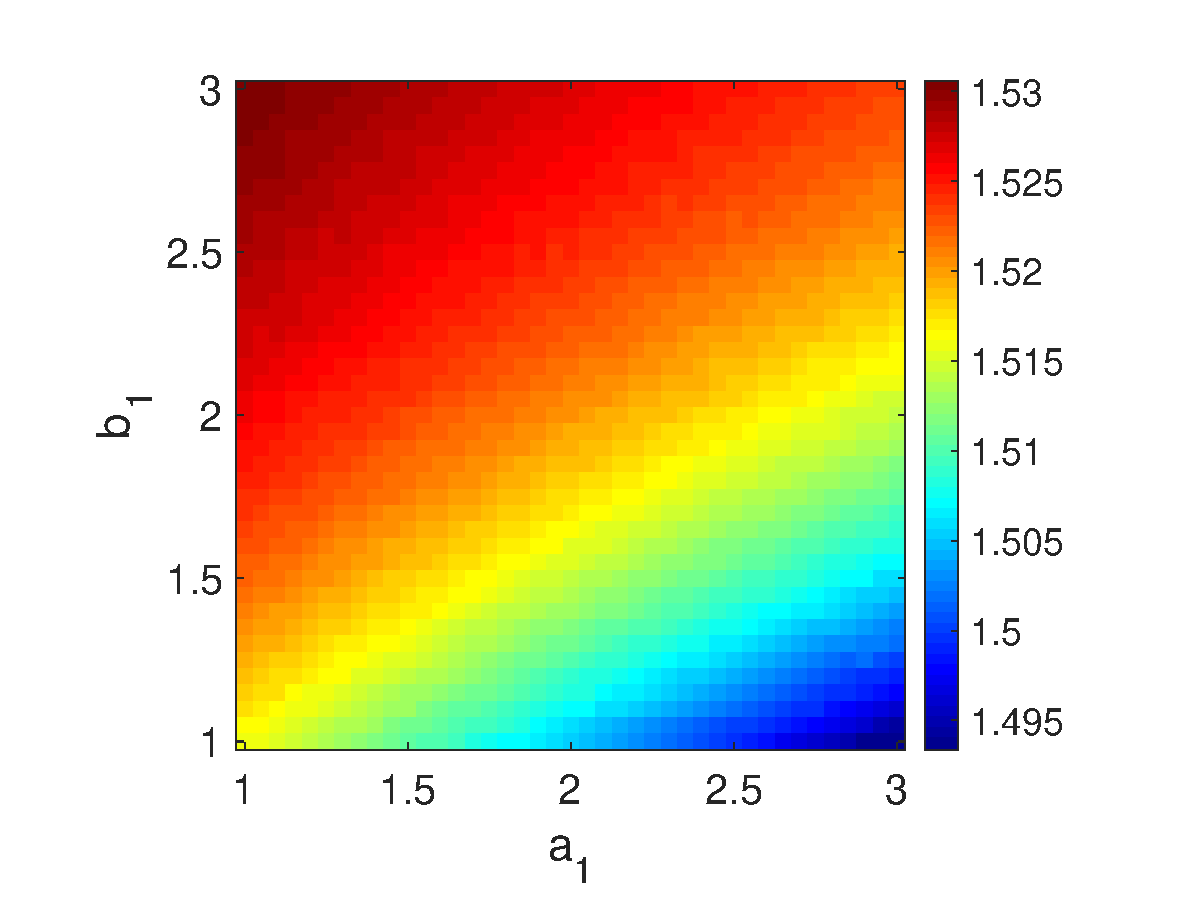
\includegraphics[width=1\linewidth]{Images/photo26_3.eps}
\end{center}

  \end{minipage} 
  
  \caption{\textbf{Total-degenerated LS on the $\lambda_{1}-b_{1}-\omega_{1}-a_{1}$ parameter space.} Both cells oscillate with amplitude value 1.5. Left and middle: LS preserving the network frequency and the amplitude of cell-1. For each pair parameters $a_{1}$ and $b_{1}$, there are the values of parameters $\lambda_{1}$ (Left) and $\omega_{1}$ (Middle), such as the amplitude value of cell-1 and the frequency network is preserved. Right: amplitude value of cell-2 for each point of the LS. Parameter values: $\lambda_{2} = 1$, $b_{2}=1$, $a_{2} = 1$, $\omega_{2} = 1$, $\alpha_{12}=2$, $\alpha_{21}=2$, $\alpha_{11}=0$ and $\alpha_{22}=0$.}
  \label{photo26}
\end{figure}

The next statement summarizes the main properties of attribute LSs on the intrinsic parameter space of a single cell.

\begin{Statement}
The two-cell network shows 2-dimensional level sets on the intrinsic parameter space of a single cell preserving the attributes (frequency and amplitude) of that cell in the network. However, the amplitude value of the other cell is not constant on each level set. Consequently, the two-cell network shows 1-dimensional total-degenerated level sets on the intrinsic parameter space of a single cell ($\lambda_{1}-b_{1}-\omega_{1}-a_{1}$ or $\lambda_{2}-b_{2}-\omega_{2}-a_{2}$ parameter spaces).
\end{Statement}

In order to gain insight on the different parameter compensations, Fig. (\ref{photo27}) shows in more detail the corresponding compensatory relations leading to total-degenerated LS on the intrinsic parameter space of a single cell.

\begin{figure}[h]
  \begin{minipage}{0.32\linewidth}
  \begin{center}
\includegraphics[width=1\linewidth]{Images/photo27_1.eps}
\end{center}
  \end{minipage} 
  \begin{minipage}{0.32\linewidth}
  \begin{center}
\includegraphics[width=1\linewidth]{Images/photo27_2.eps}
\end{center}

  \end{minipage} 
   \begin{minipage}{0.32\linewidth}
  \begin{center}
\includegraphics[width=1\linewidth]{Images/photo27_3.eps}
\end{center}

  \end{minipage} 
  
     \caption{\textbf{Total-degenerated LS on the connectivity parameter space of a single cell.} Network amplitude, $A_{\text{Net}} = 1.5$ and network frequency, $f_{\text{Net}} = 0.45$. Left: total-degenerated LS parametrized by either parameter $b_{1}$ or $a_{1}$. Black line represents the projection of compensated parameters $\lambda_{1}$ and $\omega_{1}$ onto the $a_{1}-b_{1}$ parameter space. Middle: voltage traces at the point of the LS with $\alpha_{12}=0.7$. Left: voltage traces at the point of the LS with $\alpha_{12}=2.2$. Parameter values: $\lambda_{2}=1$, $b_{2}=1$, $a_{2} = 1$, $\omega_{2} = 1$, $\alpha_{11}=0$, $\alpha_{22}=0$, $\alpha_{12}=1$ and $\alpha_{21}=1$.}
  \label{photo27}
\end{figure}

It is shown the differences on the compensatory relations between parameters. While parameters $\lambda_{1}$ and $b_{1}$ have a positive compensation (if one increases the other increases or vice versa), parameters $\omega_{1}$ and $a_{1}$ have a negative compensation (if one increases the other decreases or vice versa). This type of compensation relations was also seen at the individual neuron level, Eqs. (\ref{e16}) and (\ref{e18}). However, new dependencies are observed between parameters. More specifically, parameters $a_{1}$ and $b_{1}$ compensate each other. An increase in parameter $a_{1}$ induces an increase in parameter $b_{1}$, or vice versa. This compensatory relation is shown in Fig. (\ref{photo27})-Left (Black curve).

Moreover, Fig. (\ref{photo27}) also shows voltage traces for two different points in the total-degenerated LS considered. Some slight differences are observed, but in contrast to total-degenerated LSs on the connectivity parameter space no significant change in phase difference is observed.

\subsection{Combined parameter space}
As a final result, we consider the combined $\lambda_{1}-b_{1}-\lambda_{2}-b_{2}$ parameter space. It involves intrinsic parameters from both cells in the network. We characterize total-degenerated LSs in this parameter space.

Fig. (\ref{photo28}) shows an example of a network amplitude LS ($A_{\text{Net}}=1$) on the $\lambda_{1}-b_{1}-\lambda_{2}-b_{2}$ parameter space. It is parametrized in terms of compensating parameters $\lambda_{1}$ and $\lambda_{2}$. It is also shown the network frequency for each point on the LS. In particular, curves on the amplitude LSs preserving the network frequency represent total-degenerated LSs on the $\lambda_{1}-b_{1}-\lambda_{2}-b_{2}$ parameter space.

\begin{figure}[h]
  \begin{minipage}{0.32\linewidth}
  \begin{center}
\includegraphics[width=1\linewidth]{Images/photo28_1.eps}
\end{center}
  \end{minipage} 
  \begin{minipage}{0.32\linewidth}
  \begin{center}
\includegraphics[width=1\linewidth]{Images/photo28_2.eps}
\end{center}

  \end{minipage} 
   \begin{minipage}{0.32\linewidth}
  \begin{center}
\includegraphics[width=1\linewidth]{Images/photo28_3.eps}
\end{center}

  \end{minipage} 
  
  \caption{\textbf{Total-degenerated LSs on the $\lambda_{1}-b_{1}-\lambda_{2}-b_{2}$ parameter space.} Both cells oscillate with amplitude value 1. Left/Middle: amplitude LS on the $\lambda_{1}-b_{1}-\lambda_{2}-b_{2}$ parameter space. For each pair of $\lambda_{1}$ and $\lambda_{2}$, there are the values of parameters, $b_{1}$ (Left) and $b_{2}$ (Middle), such as the amplitude of each cell is preserved. Right: frequency in each point in the amplitude LS. Parameter values: $a_{1} = 1$, $\omega_{1} = 1$, $a_{2} = 1$, $\omega_{2} = 1$, $\alpha_{12} = 1$, $\alpha_{21} = 1$, $\alpha_{11} = 0$ and $\alpha_{22} = 0$.}
  \label{photo28}
\end{figure}

The next statement summarizes the main properties of network total-degenerated LSs on the $\lambda_{1}-b_{1}-\lambda_{2}-b_{2}$ parameter space.

\begin{Statement}
Two-cell networks show 1-dimensional total-degenerated level sets on the $\lambda_{1}-b_{1}-\lambda_{2}-b_{2}$ parameter space. Furthermore, total-degenerated level sets are closed curves.
\end{Statement}

Interestingly, when considered a combined parameter space involving intrinsic parameter from both cells in the network, closed curves representing total-degenerated LSs are found.